\documentclass[12pt]{report}

\usepackage[magyar]{babel}
\usepackage{pdfpages}
\usepackage{cite}
\usepackage{graphicx}
\graphicspath{ {./Abrak/} }
\usepackage{float}
\usepackage{listings}
\usepackage{xcolor}
\usepackage{caption}
\usepackage{amsmath}
\usepackage{geometry}

\geometry{
 left=30mm,
 top=25.4mm,
 right=25.4mm,
 bottom=25.4mm
 }
 \linespread{1.5}

\lstset{	
    frame=single,
    language=c++,
    tabsize=4,
    showstringspaces=false,    
    commentstyle=\color{green},
    keywordstyle=\color{blue},
    stringstyle=\color{red}
}

\begin{document}


\includepdf[pages = {1-4}]{kezdo_oldalak.pdf}
\pagenumbering{gobble}
\tableofcontents
\clearpage
\pagenumbering{arabic}
\chapter{Bevezetés}
Az ütemezés feladatával az élet számos területén találkozunk, kezdve az egyszerű, hétköznapi problémáktól, mint például egy napon elvégzendő feladataink sorrendjének beosztása, professzionális sportcsapatok heti edzésprogramjának kialakításán át, egészen az ipari üzemek működéséig, ahol a rendelkezésre álló berendezésekhez kell rendelni az előállítani kívánt termékeket. Bár az életünk különböző területein fellépő ütemezési problémák különböznek egymástól, bizonyos mértékben hasonlóság is fellelhető közöttük. Eltérés lehet az ütemezési feladatok célfüggvénye, valamint az adott ütemezési probléma lehet online, offline, illetve sztochasztikus vagy determinisztikus. Minden fellépő probléma esetében az a cél, hogy az elvégzendő feladatokat a rendelkezésre álló erőforrások között megosszuk oly módon, hogy adott intervallumon belül a lehető legjobb megoldást kapjuk. Fontos az, hogy ezt úgy tegyük meg, hogy a folyamat során fellépő korlátokat betartjuk, azokat nem sértjük meg. Az ipari ütemezés két leggyakoribb célja a makespan minimalizálás, és a throughput maximalizálás. A szakirodalomban legtöbb esetben a \textit{makespan} kifejezést az idő minimalizálására, a \textit{throughput} kifejezést pedig a termelés során előállított mennyiség maximalizálására alkalmazzák.

Az ipari gyártási folyamatok ütemezésére különböző módszerek léteznek már. Ezek közé tartoznak a MILP (Mixed Integer Linear Programming - vegyes egészértékű lineáris programozás) megoldó módszerek, amelyek a lineáris programozáson alapulnak. Továbbá ide sorolható az időzített automaták, Petri hálók, valamint a S-gráf megoldó módszer, amely a munkám során a legfontosabb szerepet tölti be a felsorolt megoldó módszerek közül. Dolgozatom második fejezetében ezek a módszerek kerülnek bemutatásra. A harmadik részben a problémát definiálása történik meg. A negyedikben az általam megvalósított módszer elmélete található. Az ötödik fejezetben a módszer megvalósítását és szoftverbe való beillesztését mutatom be. A hatodik fejezetben tesztelésről, és az eredmények összehasonlításáról lesz szó. A dolgozat végén található az összefoglalás a munkámról, a hivatkozások, valamint a függelék.
\chapter{Irodalmi áttekintés}
\section{Ipari ütemezési feladatok}
Az ipari folyamatok közé tartozó tevékenységeknek egy jelentős halmazát gyártásnak nevezzük, amely során az elkészítendő termék létrehozása, megvalósítása a feladat. Ehhez szükség van arra, hogy megfelelően vegyük igénybe a rendelkezésre álló erőforrásokat, amelyeket berendezéseknek, unitnak nevezünk a gyártási feladatok során. A folyamat során fellépő feladatokra a taszk elnevezés is használható. Az ütemezés az a folyamat, amely során különböző események sorrendjét határozzuk meg. Az ütemezési feladat során kell egy feladatot, munkát vagy tevékenységet egy tervbe beilleszteni, vagyis meghatározni annak végrehajtási időpontját. Minden ütemezési feladat rendelkezik végrehajtási idővel, ami megmutatja mekkora időtartam alatt valósítható meg. Ezenfelül lehet még a feladatoknak olyan időkorlátja, ami alatt kötelező elvégezni a feladatot, ezt időhorizontnak, time horizontnak hívjuk. A problémák kimenetelük szerint lehetnek megvalósíthatatlan (infeasible) és megvalósítható (feasible) feladatok.
Egy feladat csak abban az esetben minősül megvalósíthatónak, ha minden korlátozásnak megfelel. Ha már akár csak egy korlátozással szemben nem bizonyul elfogadhatónak, akkor infeasible feladatról beszélhetünk.

Az ipari folyamatokat többféleképpen lehet csoportosítani. Az egyik felosztási módszer szerint folyamatos és szakaszos üzemű rendszerek csoportjára bontjuk őket. Az első típusban az anyag folyamatosan kerül a rendszerbe, a másodikban pedig ez a folyamat lépésekben valósul meg. A munkám az utóbbi típusba tartozó feladatokra koncentrál. Másik lehetséges felosztás az, amikor online, offline, és semi-offline kategóriákba vannak a feladatok besorolva. Az offline esetben minden szükséges bemeneti adat rendelkezésre áll az optimalizálás idejében. Ezzel szemben az online esetben előbb kell a döntéseket meghozni, minthogy az adott paraméterekhez tartozó értékekre fény derülne. A semi-offline a kettő közé sorolható, azaz bizonyos információk, adatok már rendelkezésre állnak, mások viszont nem. 

Az ütemezési feladatok modelljét receptnek nevezzük. Egy termék receptje tartalmazza az adott recept által előállítható termék elkészítéséhez szükséges információkat\cite{Hegyhati}. Egy receptet a következő elemek közösen alkotják:
\begin{itemize}
  \item termékek listája,
  \item taszkok listája, amelyek adott sorrendben történő elvégzése szükséges a termék előállításához,
  \item termeléshez kapcsolódó taszkok sorrendje,
  \item rendelkezésre álló berendezések,
  \item a lehetséges taszk-berendezés párokhoz tartozó feldolgozási idő.
\end{itemize}
A recepteket a feladatok precedenciája szerint az alábbi csoportokba lehet besorolni. A felsorolás a legegyszerűbbtől halad az általánosabb felé. Minden osztály a következőnek egy speciális esete.
\begin{itemize}
	\item \textbf{Single Stage:} Egy lépésben állítható elő minden egyes termék.
	\item \textbf{Simple Multiproduct:} Minden terméket meghatározott számú fázison, szakaszon keresztül lehet elkészíteni. Előzővel szemben itt már nem csak egy lépésben lehetséges. Különösen fontos, hogy nem lehet elágazás benne, azaz csak szekvenciális lehet.
	\item \textbf{General Multiproduct:} Előzővel összehasonlítva az a különbség, hogy ennél lehetséges lépések kihagyása.
	\item \textbf{Multipurpose:} Megegyezik a Multiproduct esettel, azzal a különbséggel, hogy a berendezéset nem azonos sorrendben kerülnek igénybe vételre.
	\item \textbf{Precedential:} Egy termék gyártása nem szükségszerűen lineáris, lehetnek elágazások, kör azonban nem megengedett. Minden taszk előfeltételét be kell fejezni mielőtt az adott lépés megkezdődik. 
	\item \textbf{General Network:} A legáltalánosabb recept, ahol a taszkok a bemenetük és a kimenetük által adottak. Ilyen esetben kör is lehetséges.
\end{itemize}
Néhány előbb említett feladattípus szemléltetése látható a~\ref{receptek} ábrán. A receptek jobb oldalán lévő, T-vel jelölt kör reprezentálja a terméket, a többi pedig a taszkokat.
\begin{figure}[H]	
\begin{center}
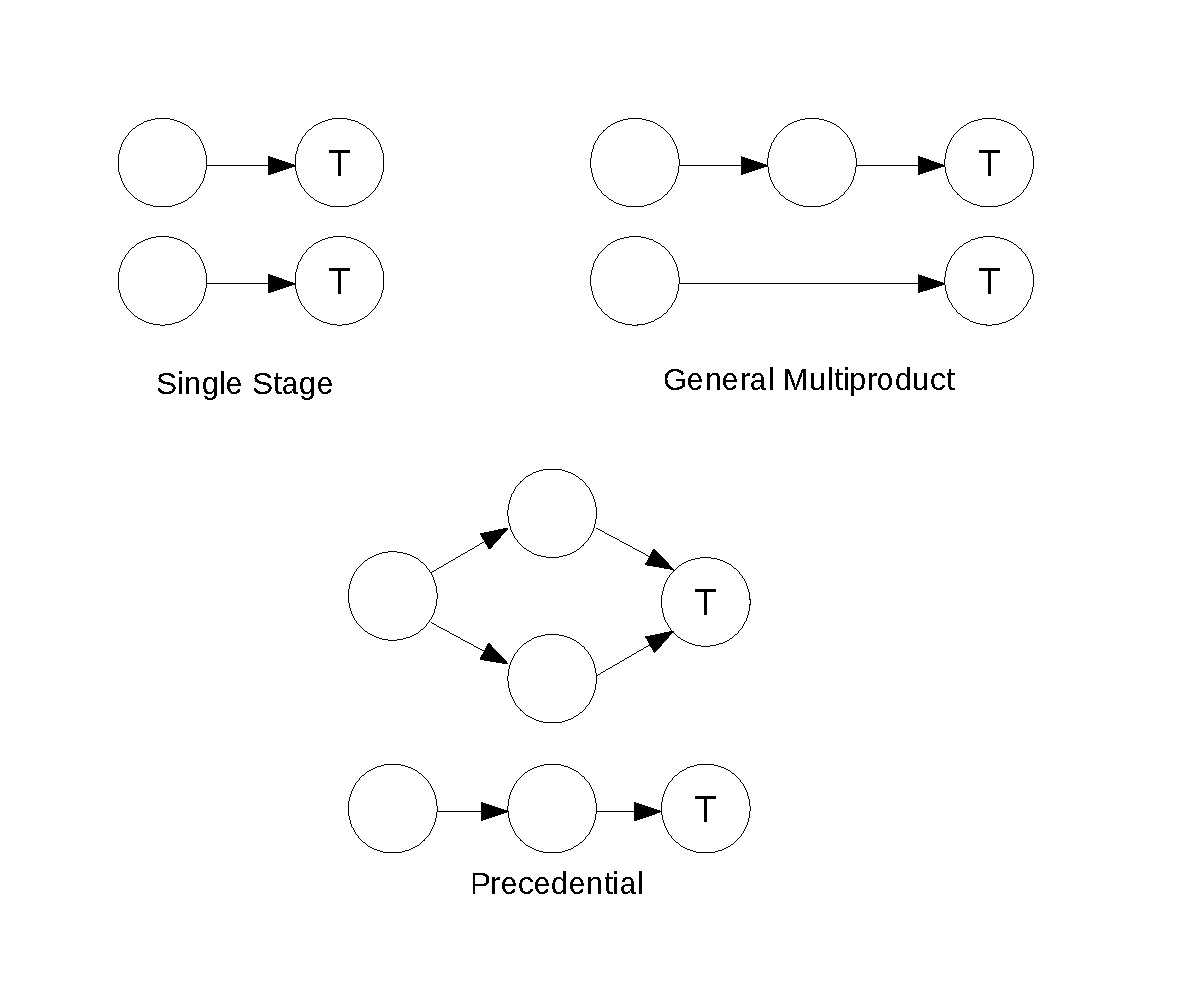
\includegraphics[scale=0.7]{receptek}
\caption{Különböző receptek szemléltetése}
\label{receptek}
\end{center}
\end{figure}
\newpage
A vegyipari, gyártási ütemezési feladatoknál nagy szerepet játszik a tárolási irányelv, amely azt mutatja meg, hogy két egymást követő feladatok között az elkészített köztes termékeket, hogyan kell raktározni, tárolni, illetve ez mennyi ideig lehetséges. A tárolási irányelvek csoportosítására többféle lehetőség van. Egyik ezek közül, amikor az adott létesítmény infrastrukturális képességei korlátozzák az anyag mennyiségét és tárolásának módját.
\begin{itemize}
	\item \textbf{UIS - Unlimited Intermediate Storage}
	\item \textbf{FIS - Finite Intermediate Storage}
	\item \textbf{NIS - No Intermediate Storage}
\end{itemize}
Az UIS eset a legmegengedőbb. Ebben az esetben van lehetőség a köztes anyagok bármely mértékű tárolására. FIS esetben van lehetőség a tárolásra, de csak korlátozott mennyiségben. A NIS esetében nincs külön tárolásra alkalmas egység, de az megoldható, hogy amíg a következő feldolgozó egységhez kerül, addig az előző taszk feldolgozó egységében várakozzon.	

A tárolás második fajta csoportosításának alapját az idő adja, amely a köztes termék kémiai és fizikai tulajdonságait befolyásolhatja. Például a termék szavatossága, hőmérséklete megfelelő maradjon a következő részfeladat elkezdéséig.	
\begin{itemize}
	\item \textbf{UW - Unlimited Wait}
	\item \textbf{LW - Limited Wait}
	\item \textbf{ZW - Zero Wait}	
\end{itemize}
ZW esetben nincs lehetőség a köztes anyag tárolására, azaz ha a berendezés befejezte a munkát, akkor azonnal folytatni kell a gyártást. Az LW esetben van egy idő, amíg a köztes termék várakozhat. Azonban, ha ez a rendelkezésre álló idő elfogy, akkor muszáj folytatni a gyártás folyamatát. Az UW eset a legmegengedőbb mind közül, ugyanis ha a köztes anyag tulajdonságai lehetőséget biztosítanak, akkor a tárolási idő nincs korlátozva, bármennyi ideig lehetőség van a tárolásra, raktározásra.
\newpage
\section{Megoldó módszerek}
Az ütemezési feladatok megoldására számos megoldó módszer létezik. Ezek közül a legismertebbek, és legszélesebb körben elterjedt módszerek kerülnek bemutatásra a dolgozatom következő pontjaiban.
\subsection{MILP modellek}
Az egyik legszélesebb körben elterjedt modell a \textbf{M}ixed \textbf{I}nteger \textbf{L}inear \textbf{P}rogramming, azaz a vegyes egészértékű lineáris programozás. Az ilyen modellekben vegyesen fordulnak elő folytonos és egész változók. Több altípus létezik:
\begin{itemize}
  \item[] \textbf{Időfelosztásos modellek - Time discretization based:} A módszer időpontokat és időréseket határoz meg. Ezek a modellek jelentek meg legkorábban kronológiailag \cite{kondili}. Az időrésen és az időponton alapuló megközelítések sok hasonlóságot mutatnak, mivel egy időintervallumtól egy másikig terjedő időintervallumot tekinthetünk időrésnek \cite{susarla}. Ellenkező irányból nézve pedig egy időrés kezdő időpontját tekinthetjük egy időpontnak.  
  
Minden időpontban bináris változók vannak hozzárendelve a feladatokhoz aszerint, hogy az adott időpillanatban elkezdődik a feladat végrehajtása vagy sem. A bináris változók száma arányos lesz a kiválasztott időpontok számával, ezért a megoldáshoz szükséges idő nagy mértékben függ az időpontok számától. Mindig megvolt a szándék olyan módszer kifejlesztésére, amelyben a szükséges időpontok száma minél kisebb legyen amellett, hogy megtalálja az optimális megoldást. Létrejöttek jobb modellek, azonban készültek olyanok is, amelyek kevésbé voltak átláthatóak, a korlátozások még bonyolultabbá váltak, és modellezési hibák is előfordultak.
  
  \item[] \textbf{Precedencia alapú modellek - Precedence based:} Ezeknél a módszereknél, szemben az időfelosztásos módszerekkel, nincs szükség az időhorizont diszkretizáció- jára, azaz nem használnak ismeretlen paramétert a modellben. Általánosságban jobb számítási eredményeket nyújtanak az általuk kezelt problémákra, azonban ez a készlet sokkal kisebb, mint az időfelosztásos modellekhez tartozó kollekció. Alapvetően a multiproduct és multipurpose receptek esetében használható megfelelően, de kibővíthető, hogy a sokkal általánosabb precedential receptek is megoldhatók legyenek ezek segítségével. 
  
Ez a módszer kettő darab bináris változót használ. Az első $Y_{i,j}$, aminek az értéke abban az esetben lesz 1, ha $i$ feladatot $j$ berendezés végzi el. A második változó: $X_{i,j,i'}$. Értéke akkor lesz 1, ha ugyanaz a berendezés végzi el az $i$ és $i'$ taszkot, méghozzá úgy, hogy előbb az $i$-t teljesíti. 
\end{itemize}
\subsection{Analízis alapú eszközök}
Az automatákat és Petri hálókat széles körben alkalmazzák diszkrét eseményrendszerek modellezésére \cite{cassandras}. Számos kísérletet tettek ezen eszközök modellezési teljesítményének kiterjesztésére annak érdekében, hogy batch folyamatok ütemezésére is alkalmassá tegyék az említett eszközöket. A meglévő modelleket időzítéssel egészítették ki, így jöttek létre a Timed Place Petri Nets (TPPN) and Timed Priced Automata (TPA) módszerek, amelyek Branch and Bound algoritmust használnak azért, hogy a legelőnyösebb megoldást megtalálják. Ezen módszereknek a hatékonysága elmarad a MILP és az S-gráf modell hatékonyságától is.
\begin{itemize}
	\item[] \textbf{Időzített automaták:} Ezekben a megközelítésekben a recepteket és a berendezéseket külön modellezik, és a rendszer modellje ezeknek a párhuzamos összetételével jön létre. A bonyolultságot az jelenti, hogy az órák állapota végtelen lehet, és emiatt a rendszer állapotterülete is az lehet.
	\item[] \textbf{Időzített Petri háló:} Az alap ilyen módszereknél, hogy az átvitel jele késleltetés alapján jön létre. Többen is foglalkoztak a témával, például Ghaeli \cite{ghaeli}, aki batch folyamatok ütemezésével tanulmányozta.
\end{itemize}

\subsection{S-gráf módszertan}
Az S-gráf keretrendszer volt az első olyan publikált módszer, amely gráf elméleten alapult, valamint szakaszos gyártórendszerek ütemezési problémáinak megoldására szolgált \cite{combtech}. Ez a keretrendszer egy irányított gráf modellből, az S-gráfból, és a hozzá tartozó algoritmusokból áll \cite{combframe}. Az S-gráf egy speciális irányított gráf, amely ütemezési problémák számára lett létrehozva. Nemcsak a recept vizualizációja, hanem egyben matematikai modell is. A keretrendszerben az S-gráf reprezentálja a recepteket, a részleges és a teljes ütemterveket is. Ezekben a gráfokban a termékeket és a feladatokat csúcsok jelölik, amelyeket csomópontoknak (node) nevezünk. Az ütemezési döntés nélküli S-gráfot \textbf{Receptgráfnak} nevezzük. Erre példa a~\ref{receptGraf} ábrán látható \cite{Hegyhati}. 
\begin{figure}[H]	
\begin{center}
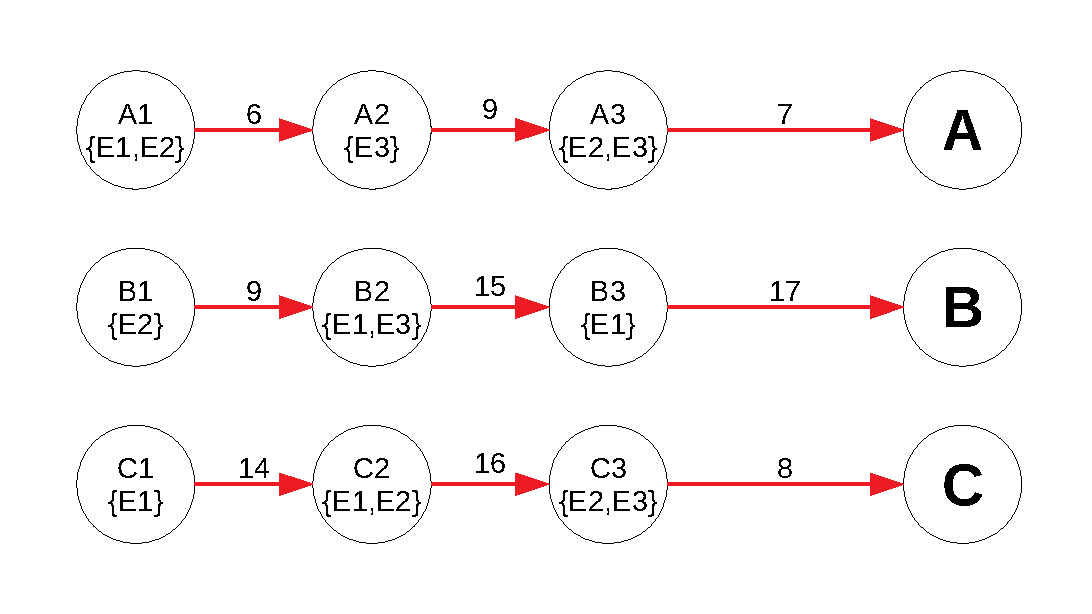
\includegraphics[scale=0.7]{receptGraf}
\caption{A receptgráf szemléltetése}
\label{receptGraf}
\end{center}
\end{figure}
A jobb oldalon látható három, nagybetűvel jelölt csomópont felel meg a termékeknek, a maradék kilenc pedig a részfeladatokat jelenti. Ezt a kilenc részfeladatot el kell végezni a termékek előállításának érdekében. Az élek a csomópontok közti függőséget mutatják meg. Ezeket \textbf{Receptéleknek} nevezzük. Kétfajta függőséget tudunk megkülönböztetni:
\begin{itemize}
  \item Két részfeladat között van él. Ebben az esetben az egyik készíti el a másiknak a bemenetét.
  \item Egy termék és egy részfeladat között szerepel él. Ilyenkor a részfeladat készíti el a terméket.
\end{itemize}
Az éleken látható súlyok a részfeladat végrehajtásához szükséges időt mutatják meg. Ha egy részfeladatot több berendezés is képes elvégezni, akkor az előbb említett súly mindig a legkisebb előállítási idő lesz.

Minden S-gráf-hoz kapcsolódó algoritmus kiegészíti ezeket a gráfokat az úgynevezett \textbf{ütemezési élekkel}, amelyek az ütemezési döntést testesítik meg. Ezekkel az élekkel kiegészített gráfoknak a neve \textbf{Ütemezési gráf}. Példa a~\ref{utemezesiGraf} ábrán nézhető meg. Az ábrán sötétkékkel jelölt élek az ütemezési élek. Az ütemezési élek súlya alapértelmezetten nulla, ha a probléma nem tartalmaz szállítási, vagy tisztítási időt. A részfeladatok csomópontjain már nem a lehetséges berendezések halmaza látható, hanem egy konkrét kiválasztott berendezés, az ütemezési döntésnek megfelelően. 
\begin{figure}[H]
\begin{center}
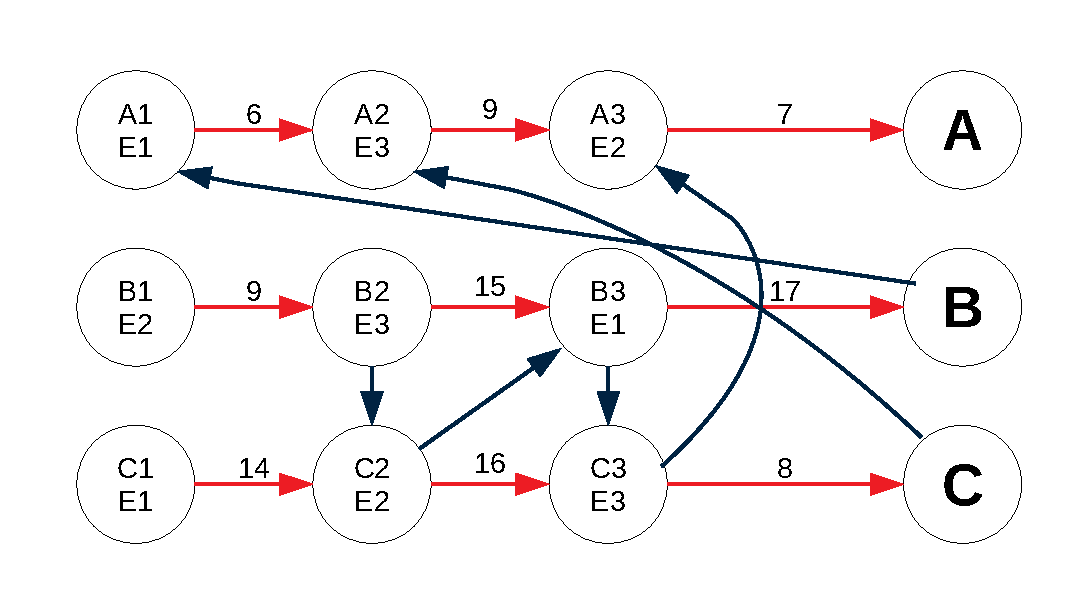
\includegraphics[scale=0.7]{utemezesiGraf}
\caption{Az ütemezési gráf szemléltetése}
\label{utemezesiGraf}
\end{center}
\end{figure}
Ugyanahhoz a berendezéshez rendelt részfeladatok végrehajtási sorrendje könnyedén leolvasható a gráfról. A~\ref{utemezesiGraf2} ábrán látható példában az E2-es berendezés által elvégzett részfeladatok sorrendje B1 $\to$ C2 $\to$ A3. Az ütemezési él azt mutatja meg, hogy nem elég az, hogy az E2 berendezés végrehajtsa a B1 feladatot, hanem ezt a közbenső terméket a B2 feladathoz tartozó E3 berendezés átvegye. Csak ezeket követően tudja megkezdeni az adott részfeladat végrehajtását.
\begin{figure}[H]
\begin{center}
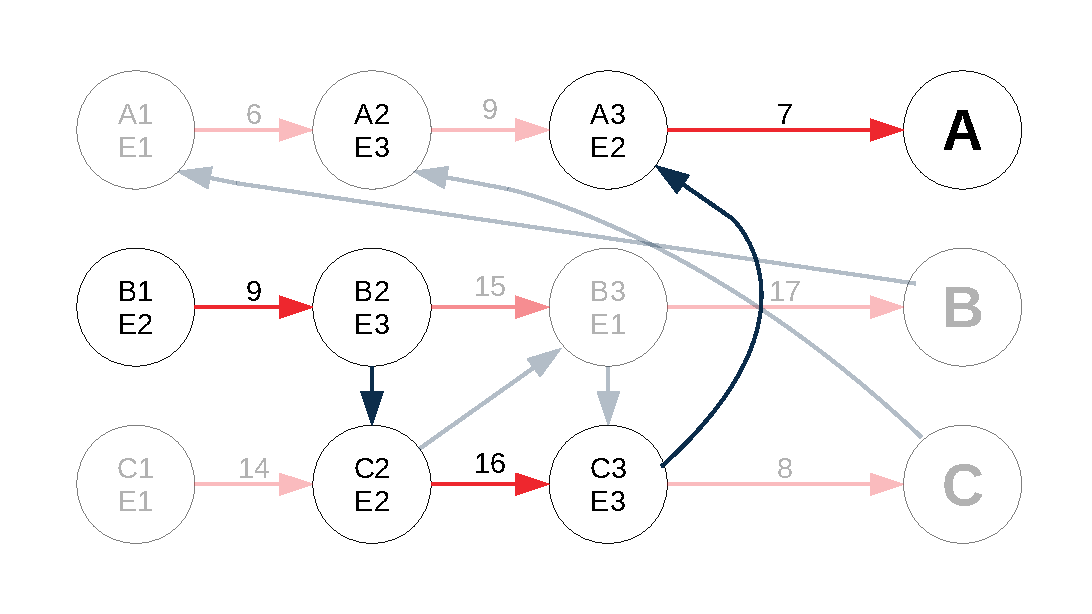
\includegraphics[scale=0.7]{utemezesiGraf2}
\caption{E2-es berendezés által elvégzett részfeladatok}
\label{utemezesiGraf2}
\end{center}
\end{figure}
Gyakran használt mód az ütemezési feladatok ábrázolására a Gantt diagram\cite{ganttwwf}, \cite{ganttofw}. Ezeken a diagramokon a függőleges tengelyen a berendezések, míg a vízszintes tengelyen pedig az idő szerepel. Az ábrán látható erőforrások szemléltetik az erőforrások elfoglaltságát. Egy Gantt diagram látható a~\ref{GanttDiagram} ábrán.
\begin{figure}[H]
\begin{center}
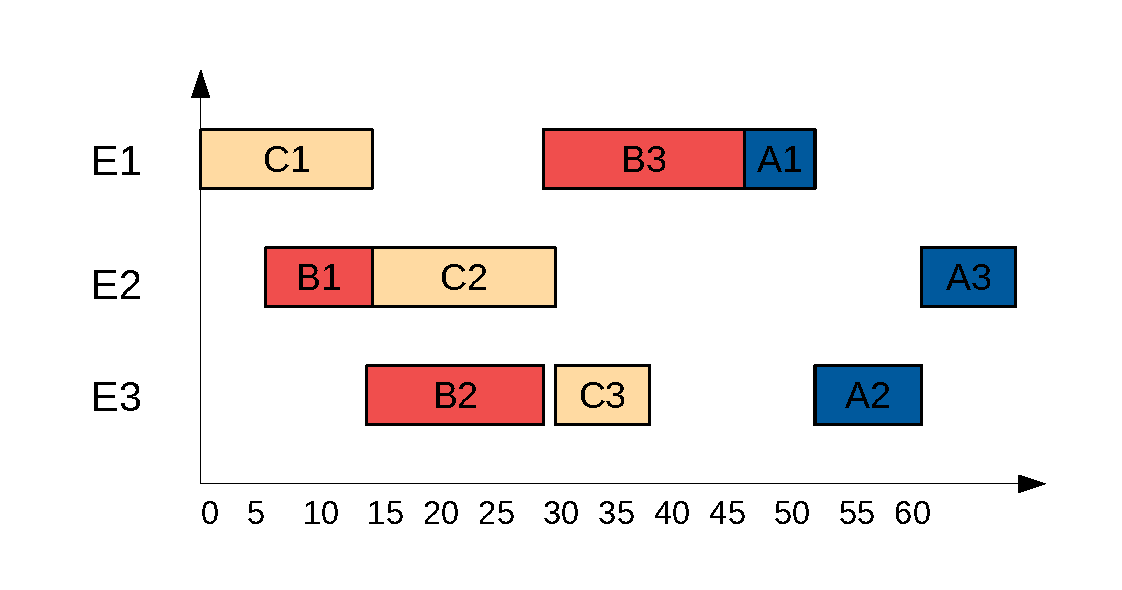
\includegraphics[scale=0.7]{GanttDiagram}
\caption{Egy ütemezés Gantt diagramon való megjelenítése}
\label{GanttDiagram}
\end{center}
\end{figure}

\subsection{A makespan minimalizálás algoritmusa}
Az egyik legelső célja az S-gráf keretrendszer létrehozásának a makespan minimalizálás volt. Ennek alapja egy Branch \& Bound algoritmus, amivel lehetséges a termékek előállítási idejét minimalizálni.

Az algoritmus első lépésben inicializálja a $makespan^{cb}$ értékét végtelennel, majd beállítja az $S$ halmazt, amelyben az ütemezés során a nyitott részproblémák szerepelnek. Kezdetben csak a gyökér probléma szerepel benne, vagyis egy receptgráf bármilyen hozzárendelés nélkül. A \textbf{recipe} függvény visszaadja a probléma receptgráfjának modelljét, amit a $G(N,A_1,A_2,w)$ jelöl, amiben:
\begin{itemize}
	\item $N:$ a csomópontok halmaza (termékek és taszkok együttese)
	\item $A_{1}:$ a receptélek halmaza
	\item $A_{2}:$ az ütemezési élek halmaza (itt még üres halmaz)
	\item $w_{i,i^{'}}:$ a receptélekhez tartozó súlyok, amelyek az $i$ taszkok legkisebb feldolgozási idejét jelentik.
\end{itemize}

Az iteráció minden lépésében a \textbf{select\_remove} függvénnyel egy tetszőleges részprobléma kerül kiválasztásra, majd az $S$-ből eltávolításra. Ennek a függvénynek a viselkedése a különböző megvalósításokban más és más lehet, ami más keresési stratégiát eredményez. A kiválasztott részprobléma a következőképpen néz ki $(G(N,A_1,A_2,w),I',J',{\cal A})$, ahol:
\begin{itemize}
	\item $G(N,A_{1},A_{2},w):$ az ütemezési gráf
	\item $I^{'}:$ a még nem ütemezett taszkok halmaza
	\item $J^{'}:$ azon berendezések halmaza, amelyekhez az algoritmus még tud rendelni taszkokat 
	\item $\cal{A}:$ taszk-berendezés hozzárendelések halmaza, $(i,j)$ párok formájában 
\end{itemize}

Az iteráció elején kiértékelődik, hogy a részprobléma képes-e egy optimális megoldást nyújtani vagy sem. Ez a \textbf{bound} függvénnyel történik. Ezzel szemben több követelmény áll fenn. Alsó korlátot kell adnia azoknak a megoldásoknak, amelyek a részproblémából származnak. Biztosítania kell levél problémák pontos makespanjét. Végtelen értékkel térjen vissza, ha a gráf tartalmaz kört, és jelezze, hogy megoldhatatlan. A leggyakrabban a leghosszabb út keresésével vizsgálja meg a részproblémát a \textbf{bound} függvény, de lehetséges LP alapú modellek használata is.

Ha a korlát nem kisebb, mint az eddig megtalált legjobb eredmény, akkor az iteráció véget ér, és amennyiben létezik egy következő részprobléma, akkor az kerül kiválasztásra.
Ha viszont kisebb a korlát, abban az esetben ellenőrzi az algoritmus azt, hogy az összes taszk már ütemezett-e, vagyis a még nem ütemezett taszkok halmaza üres már ($I^{'}=\emptyset$). Ha így van frissül a legjobb megoldás gráfja, a legjobb makespan és a hozzárendelések halmaza. Ellenben, ha még szükséges további ütemezés, akkor a  \textbf{select} függvény kiválaszt egy rendelkezésre álló berendezést a $J^{'}$ halmazból. A kiválasztott $j$ berendezéshez az algoritmus hozzárendeli az összes lehetséges taszkot a még nem ütemezett taszkok és a kiválasztott berendezés által elvégezhető taszkok közös halmazából ($i \in I_{j} \cap I^{'}$). Ezek a kiválasztott taszkok kapnak egy másolatot az aktuális S-gráfról. Mivel a csomópontok és a receptélek halmaza nem változik, ezért ezek változatlanok maradnak, csak az ütemezési élek halmaza és súlyok változnak. Ezt a másolatot kibővíti az algoritmus az új hozzárendelés alapján az ütemezési élekkel ($A^{i}_{2}:= A^{i}_{2} \cup \{(i^{'},i)\}$). Ezután minden $i$-ből induló receptél súlya frissül a $t^{pr}_{i,j}$ értékével. Végezetül pedig az új részproblémát hozzáadja az $S$ halmazhoz. Itt $I^{'}$ halmazból kikerül az előbb kiválasztott $i$ taszk, és a hozzárendelések halmazába bekerül az új taszk-berendezés pár (${\cal A}\cup\{(i,j)\}$).

Abban az esetben, ha minden még nem ütemezett taszkot a kiválasztott $j$ berendezésen kívül más berendezés is el tud végezni, akkor egy új részproblémát hoz létre az algoritmus, amelyben a $j$ berendezés már nem végez több taszkot, azaz kikerül a még rendelkezésre álló berendezések halmazából ($J^{'}\setminus\{j\}$).

Ha az $S$ halmaz üres lesz, akkor a $G^{cb}$ gráf és a hozzárendelések a ${\cal A}^{cb}$ halmazban leírják az optimális megoldást. Ha legalább egy megvalósítható, akkor az algoritmus visszatér ezzel az értékkel, ellenkező esetben nem ad vissza megoldást.

\section{Throughput maximalizálás}
Eredetileg az S-gráf keretrendszer makespan minimalizációs problémák megoldására lett létrehozva, azonban a későbbiekben bővítésre került, így ezután throughput, profitmaximalizációs problémák megoldására is alkalmazhatóvá vált. Az alapötlet Majozi és Friedler \cite{majozifriedler}, valamint Holczinger és társai \cite{holczinger} nevéhez fűződik. A termékek lehetséges batch darabszámai alapján az algoritmus konfigurációkat hoz létre. A konfiguráció tehát az, ami megmutatja, hogy egy termékből hány batch készül el.
\begin{figure}[H]
\begin{center}
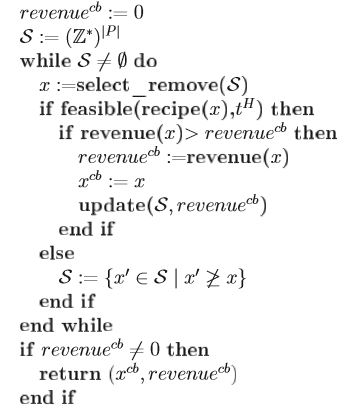
\includegraphics[scale=1]{throughput_alg}
\caption{A throughput maximalizáló algoritmus pszeudó kódja \cite{Hegyhati}}
\label{throughput_alg}
\end{center}
\end{figure}
Az algoritmus először inicializálja az $S$ halmazt a termékekre vonatkozóan minden lehetséges batch számmal. Fontos kiemelni, hogy ebben az esetben minden terméknél a batch méret rögzített, azaz egy termék batch-jének jövedelme ismert. Ezt követően minden iteráció során az előbb említett halmazból kiválasztásra kerül egy konfiguráció a \textbf{select\textunderscore remove} függvény segítségével. Ezután sor kerül a feasibilitás tesztre, amely során eldől, hogy a megadott időhorizont alatt megvalósítható vagy sem. Ha megvalósítható és nagyobb jövedelmet biztosít, mint az eddig megtalált legnagyobb jövedelem, akkor a jelenlegi legjobb megoldás és az S halmaz frissül. Ha infeasible a kiválasztott konfiguráció, akkor ez, és minden ennél nagyobb konfiguráció eltávolításra kerül az S halmazból. Amint az S halmaz üressé válik, és volt feasible megoldás, akkor az algoritmus visszatér a legjobb konfigurációval, és az ehhez tartozó jövedelem mennyiségével.

A~\ref{throughput1} ábrán látható egy Throughput módszerrel megvalósított feladat eredménye.
\begin{figure}[H]
\begin{center}
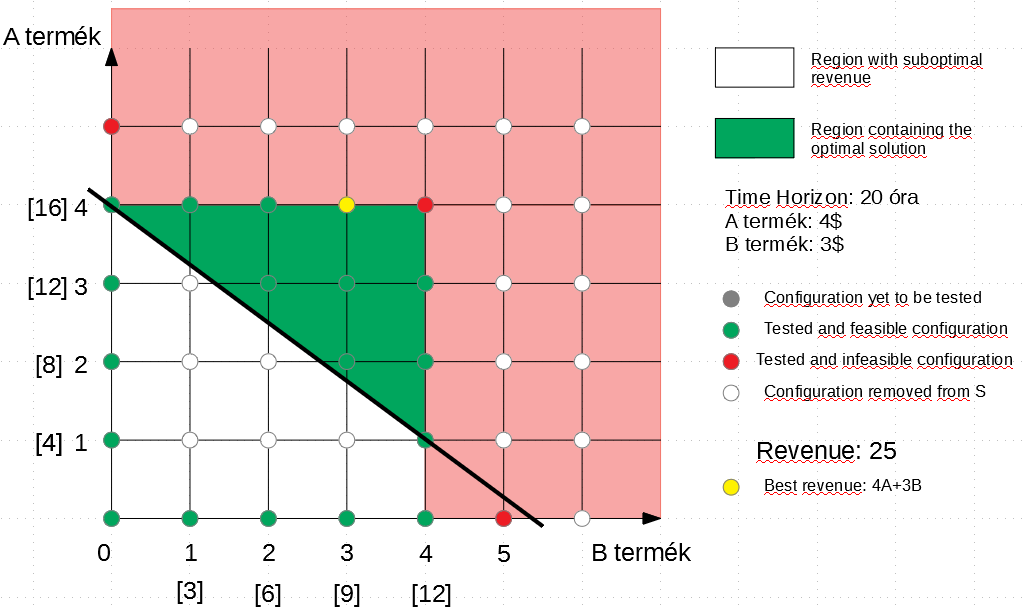
\includegraphics[scale=0.7]{throughput1}
\caption{Throughput maximalizálás szemléltetés}
\label{throughput1}
\end{center}
\end{figure}
Két termék esetén koordináta rendszeren szemléltethető az algoritmus működése. Egyik tengelyen az egyik termék, a másikon pedig a másik termék szerepel. Kezdetben az összes konfigurációt tartalmazta a konfigurációk halmaza. Az algoritmus először végighaladt az egyik tengely mentén, vagyis az egyik termék batch mérete 0 volt, a másik pedig növekedett. Ezt a haladási irányt addig követte amíg megtalálta az első nem megvalósítható, azaz infeasible konfigurációt. Ezt követően elvégzi a keresést a másik tengelyen is. Így kapott egy jelenleg maximális jövedelmet. Az utolsó még feasible batch számoknál nagyobb batch számokat már nem kell vizsgálni, hiszen azokat a megadott időhorizonton belül nem lehet megvalósítani. A képen látható feladatban a legnagyobb elérhető profit 16 volt. A feketével jelzett egyenes tartalmazza az összes 16 profittal rendelkező pontot. Ezt nevezzük revenue line-nak, amely segítségével csökkenthető a tesztelendő konfigurációk száma. Jelenlegi példában a B termékhez tartozó 16-os érték nem egész batch számhoz tartozik, a legközelebbi 15 profittal rendelkezik, ami infeasible már. Az egyenes alatt azok a konfigurációk szerepelnek, amelyek jövedelme nem éri el a jelenlegi maximumot, így ezek nem a lehető legjobb megoldást adják meg. Az algoritmus addig nem állt le , amíg a halmaz, amely a konfigurációkat tartalmazza ki nem ürül. A példafeladatban a maximálisan elérhető jövedelem 25 egység. Ezt 4 darab A termék és 3 darab B termék legyártásával lehet elérni.
\chapter{Probléma definíció}
Az előző fejezetben bemutatott throughput maximalizálás esetében kikötés volt, hogy minden termék batch mérete rögzített legyen, azaz a termékek batch-jének jövedelmét ismerjük.
Abban az esetben minden taszkhoz egy berendezés hozzárendelése megengedett, azaz csak egy berendezés végezheti el.
Azonban számos esettanulmány és irodalmi példa esetében a batch méretek nem rögzítettek.
Ha több berendezés képes elvégezni ugyanazt a taszkot, akkor ezt megtehetik párhuzamosan.
Ilyen eset főleg a throughput maximalizálás során léphet fel, de megjelenhet makespan minimalizálásnál is.
Az időfelosztásos módszerek meg tudják oldani az ilyen problémákat, azonban az S-gráf keretrendszer esetén néhány módosítás szükséges.
A throughput maximalizálás algoritmusa megköveteli, hogy a recept rögzített, valamint egy termék batch-jének jövedelme is előre ismert legyen.
Az előbb említett problémák esetén viszont egyik sem garantált. 
A javasolt megközelítés szemléltetésére a Kondili és munkatársaitól származó példát veszem igénybe \cite{kondili}.
Ez látható \ref{kondiliPelda} ábrán.

A folyamat 5 taszkból áll: fűtésből, 3 darab reakcióból, és az szétválasztásból.
Ezekhez 4 berendezés áll rendelkezésre: a fűtőtest és szeparátor, mindkettő 100 kilogrammos kapacitással a fűtés és elválasztás folyamatához.
A három reakciós folyamathoz van 2 darab reaktor ugyanakkora feldolgozási idővel.
A kapacitásuk eltér, egyiké 80 kilogramm a másiké pedig 50 kilogramm, de ezeket a reaktorokat párhuzamosan is igénybe lehet venni.
Feltételezzük, hogy az összes egység képes a kapacitásuknál kisebb terheléssel működni, azaz nincs meghatározva, hogy minimálisan mekkora mennyiség szükséges.
A folyamat során két termék készül azonos profittal.
A következő korlátozások fennállnak: nem marad semmilyen köztes anyag a termelő folyamat végén, nem lehet csak az egyes számú terméket gyártani, illetve nincs tárolásra lehetőség a folyamat során.
\begin{figure}[H]
\begin{center}
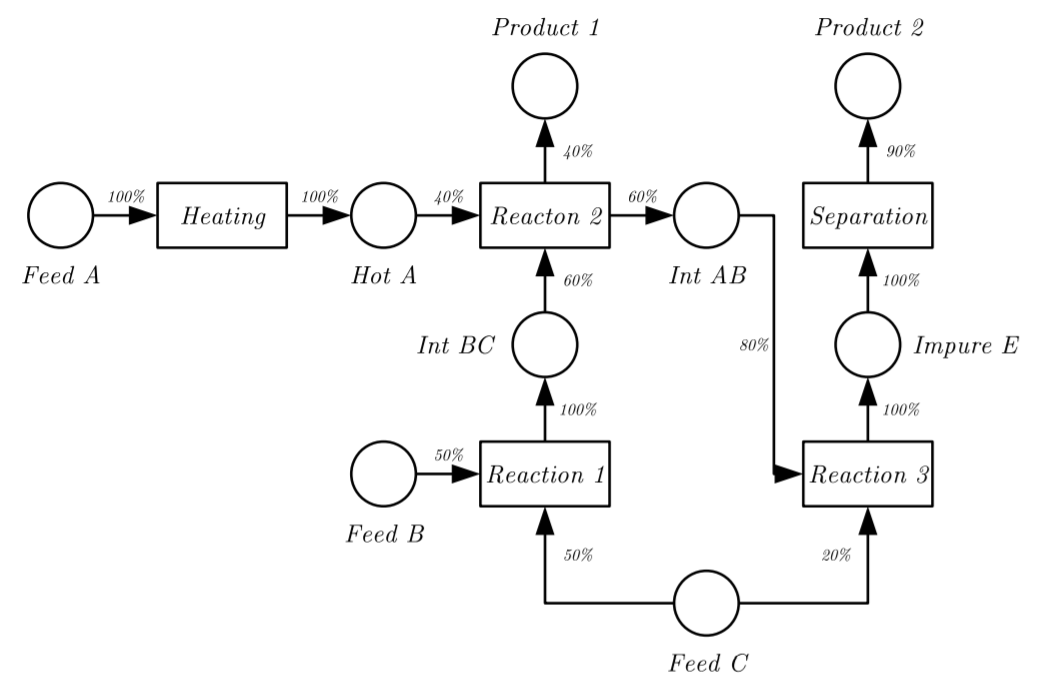
\includegraphics[scale=0.65]{kondiliPelda}
\caption{Kondili példafeladata}
\label{kondiliPelda}
\end{center}
\end{figure}

Mindegyik reakció elvégezhető az egyik, a másik, vagy egyszerre mindkettő reaktor által párhuzamosan.
Ez $3^3 = 27$ rögzített receptet eredményez, amelyek különböző batch mérettel rendelkezhetnek.
Mindegyik esetben különálló S-gráf receptet kell létrehozni, hogy a korábban említett S-gráf algoritmust igénybe lehessen venni profit maximalizálásra, így a legfelső szinten lévő keresési terület 27 dimenziós térré válna.
Ez óriási CPU igényhez vezetne az optimalizálás során, ezért az esetek számának csökkentése elengedhetetlen.

Ha megnézzük a \ref{tabla1} táblázatot, észrevehető, hogy csupán néhány érték ismétlődik.
Ennek oka az anyagok egyensúlyából származik.
Például, hogy ha mind az R1-et mind az R2-t hozzárendeljük a hármas számú reakcióhoz ahelyett, hogy csak az R1 lenne hozzárendelve, akkor sem lesz nagyobb a kimenet, mert a korábbi reakciókból származó pótlás nem éri el a szükséges szintet.
Ha a két különböző eset, $c$ és $c'$, ugyanakkora maximális jövedelemmel rendelkezik, de a $c$ eset csak kisebb részét használja a $c'$ által használt egységeknek, ekkor azt mondjuk, hogy a $c$ \textit{dominálja} a $c'$-t.
A példából látható, hogy a 9-es eset dominálja a 27-es esetet.
Továbbá a 24-es eset dominálva van a 4, 5, 6, 13, 14, 15, 22, 23 esetek által.
Megállapíthatjuk, hogy ha egy eset legalább egy másik által dominálva van, akkor azt kizárhatjuk a vizsgálatból, mert az továbbra is garantálva van, hogy megtalálja az optimális megoldást.
A \ref{tabla3} táblázat tartalmazza azokat az eseteket, amelyek nincsenek dominálva más esetek által. 

\begin{table}
	\begin{center}
		\caption{A 27 rögzített recept Kondili példájához}
		\captionsetup[table]{skip=10pt}
		\label{tabla1}
		\begin{tabular}{r|ccc|l}
		Eset & Reakció 1 & Reakció 2 & Reakció 3 & Max bevétel  \\ 
		\hline
		1    & R1        & R1        & R1        & 86,00        \\
		2    & R1        & R1        & R2        & 71,67        \\
		3    & R1        & R1        & R1\&R2    & 86,00        \\
		4    & R1        & R2        & R1        & 53,75        \\
		5    & R1        & R2        & R2        & 53,75        \\
		6    & R1        & R2        & R1\&R2    & 53,75        \\
		7    & R1        & R1\&R2    & R1        & 114,76       \\
		8    & R1        & R1\&R2    & R2        & 71,67        \\
		9    & R1        & R1\&R2    & R1\&R2    & 139,75       \\
		10   & R2        & R1        & R1        & 86,00        \\
		11   & R2        & R1        & R2        & 71,67        \\
		12   & R2        & R1        & R1\&R2    & 86,00        \\
		13   & R2        & R2        & R1        & 53,75        \\
		14   & R2        & R2        & R2        & 53,75        \\
		15   & R2        & R2        & R1\&R2    & 53,75        \\
		16   & R2        & R1\&R2    & R1        & 89,58        \\
		17   & R2        & R1\&R2    & R2        & 71,67        \\
		18   & R2        & R1\&R2    & R1\&R2    & 89,58        \\
		19   & R1\&R2    & R1        & R1        & 86,00        \\
		20   & R1\&R2    & R1        & R2        & 71,67        \\
		21   & R1\&R2    & R1        & R1\&R2    & 86,00        \\
		22   & R1\&R2    & R2        & R1        & 53,75        \\
		23   & R1\&R2    & R2        & R2        & 53,75        \\
		24   & R1\&R2    & R2        & R1\&R2    & 53,75        \\
		25   & R1\&R2    & R1\&R2    & R1        & 114,76       \\
		26   & R1\&R2    & R1\&R2    & R2        & 71,67        \\
		27   & R1\&R2    & R1\&R2    & R1\&R2    & 139,75      
		\end{tabular}
	\end{center}
\end{table}

	

\begin{table}[H]
	\begin{center}
		\caption{Nem dominált esetek bevétel szerint növekvő sorrendben}
		\captionsetup[table]{skip=10pt}	
		\label{tabla2}	
		\begin{tabular}{r|ccc|l}
		Eset & Reakció 1 & Reakció 2 & Reakció 3 & Max bevétel  \\ 
		\hline
		4    & R1        & R2        & R1        & 53,75        \\
		5    & R1        & R2        & R2        & 53,75        \\
		13   & R2        & R2        & R1        & 53,75        \\
		14   & R2        & R2        & R2        & 53,75        \\
		2    & R1        & R1        & R2        & 71,67        \\
		11   & R2        & R1        & R2        & 71,67        \\
		1    & R1        & R1        & R1        & 86,00        \\
		10   & R2        & R1        & R1        & 86,00        \\
		16   & R2        & R1\&R2    & R1        & 89,58        \\
		7    & R1        & R1\&R2    & R1        & 114,67       \\
		9    & R1        & R1\&R2    & R1\&R2    & 139,75      
		\end{tabular}
	\end{center}
\end{table}

Ezután az esetszám csökkenés után is még mindig 11 esetet kellene az S-gráf algoritmusnak megvizsgálni.
Annak érdekében, hogy tovább csökkenjen ez a szám több esetet is össze lehet vonni.
Például a 4-es és 5-ös eset teljes mértékben megegyezik, azzal a kivétellel, hogy a harmadik reakciós folyamatot más reaktor végzi.
Ezt a két esetet össze lehet vonni úgy, hogy a harmadik reakciónál R1 vagy R2-es reaktor ($R1 \vee R2$) üzemel.
A \ref{tabla3} táblázatban látható a végleges összevonás eredménye.

\begin{table}[H]
	\begin{center}
		\caption{Összevont, nem dominált esetek bevétel szerint növekvő sorrendben}
		\captionsetup[table]{skip=10pt}	
		\label{tabla3}	
		\begin{tabular}{r|ccc|l}
		Eset      & Reakció 1~ & Reakció 2 & Reakció 3 & Max bevétel  \\ 
		\hline
		4,5,13,14 & $R1 \vee R2$      & R2 & $R1 \vee R2$     & 53,75        \\
		2,11      & $R1 \vee R2$      & R1        & R2        & 71,67        \\
		1,10      & $R1 \vee R2$      & R1        & R1        & 86,00        \\
		16        & R2         & R1\&R2    & R1        & 89,58        \\
		7         & R1         & R1\&R2    & R1        & 114,67       \\
		9         & R1         & R1\&R2    & R1\&R2    & 139,75      
		\end{tabular}
	\end{center}
\end{table}

Látható, hogy az ilyen típusú feladatoknál nem lehet közvetlenül a megoldó programot igénybe venni a feladat megoldásához, szükség van előzetes lépésekre, hogy megfelelő formába kerüljön a feladat.
Ez mindig plusz időbe kerül, és ez az idő annál nagyobb lehet, minél több taszk és berendezés szerepel az adott feladatban.
A következő fejezetben bemutatott új módszer esetén ezek a lépések elhagyhatóak, ezáltal időt lehet megspórolni.
\chapter{Az új módszer}
Az új módszer létrehozását a meglévő megoldónál fellépő, a változó batch mérettel rendelkező feladatokból származó hátrányok ihlették. Abban az esetben az összes lehetséges, különböző hozzárendelést rögzíteni kell a receptben, így különböző termékek lesznek. Ennek következményeképp 1 dimenzió helyett többet kell bejárnia az algoritmusnak, ebből kifolyólag a futás lassabb lesz, mert több megvalósíthatósági tesztet kell elvégezni. Ezenkívül a nagyobb csúcsszám miatt nő az infeasible csúcsok száma is. Az új megoldó módszer ezen hátrányok kiküszöbölésére törekszik. 

A két módszer nem teljes mértékben tér el, vannak olyan részek benn, amelyek megegyeznek. Először is mindkét esetben $n$ dimenziós térben ($n$ a termékek száma) keresi a legnagyobb profittal rendelkező konfigurációt. Mindegyik módszer esetén sor kerül kerül a megvalósíthatóság tesztelésére, illetve ha talál egy megvalósíthatatlan konfigurációt akkor elveti ezt és az ennél nagyobbakat. 

A módszerek között eltéréseket is lehet találni. Legfontosabb eltérés, hogy az új módszer esetében egy receptnél nincs batch méret, emiatt a jövedelmek sincsenek előre meghatározva. Ezt a feladatot az ütemezést elvégző szubrutinnak kell elvégezni. Lényeges eltérés még, hogy az új módszernél nem alkalmazható a revenue line arra, hogy csökkentsük a megvizsgálandó konfigurációk számát. Itt a elérhető jövedelmet nem skaláris szorzat adja meg, mint a régi megoldó esetében (termék száma szorozva a termék jövedelmével), hanem a mennyiség is közrejátszik, így előfordulhat, hogy kisebb konfigurációk esetén nagyobb profitra teszünk szert. Ennek tekintetében lényeges az is, hogy ha talál egy részütemezés esetén megvalósítható megoldást, akkor nem tér azonnal vissza ezzel, hanem megkeresi a legjobb elérhetőt. Az új algoritmus nem csökkenti a beütemezendő feladatokat, mert engedélyezett, hogy több berendezés egyszerre végezze ugyanazt a feladatot. Ennek következtében a levél nem lehet az a részfeladat, ahol már nincs ütemezendő feladat. Ehelyett az számít levélnek, ha már minden berendezés ütemezése lezárt. Továbbá eltérés a felső korlátban is megfigyelhető. Az új módszernél a felső korlátot az adja, hogy a még elérhető berendezéseket hozzárendeli minden olyan feladathoz, amelyet az adott berendezés el tud végezni. Ezen a módon minden csúcsra meghatározza az elérhető legnagyobb kapacitást.

Az új módszernek 3 nagyobb elkülöníthető része van, amelyek bemutatása a következő pontokban található meg.

\section{Vezérlő}
A vezérlő feladata a konfigurációk kezelése. Első lépésben az algoritmus inicializálja a $profit^{cb}$ változót mínusz végtelennel. Ennek oka az, hogy ha a feladatnak van megoldása, akkor ennél az értéknél biztosan nagyobb jövedelemre lehet szert tenni. Ezt követően az $S$ halmazt inicializálja a termékek összes lehetséges konfigurációval. Ezek természetesen csak nem negatív egész számok lehetnek. Ezután az iteráció minden lépésében a \textbf{select\_remove} függvény segítségével kiválaszt egy konfigurációt. Először minden feladat esetében végigmegy azokon a konfigurációkon, ahol csak egy termék kerül legyártásra, így meghatározható egy régió, amely tartalmazza az összes megvalósítható megoldást. Az algoritmus meghívja a $MAXPROFIT$ függvényt, amely által visszaadott értéket összehasonlítja a jelenlegi legjobb megoldással. Ha jobb, mint a meglévő profit, akkor ez az új érték lesz a legjobb megtalált megoldás, és a legjobb konfiguráció is frissítésre kerül. Azonban, ha a visszakapott érték mínusz végtelen, akkor az az jelenti, hogy az adott konfiguráció esetén nincs megvalósítható megoldás, így az ennél nagyobb konfigurációk eltávolíthatóak az $S$ halmazból, mert azok között se található feasible megoldás. Miután az iteráció véget ért, és volt megvalósítható megoldás, akkor az algoritmus visszatér a legjobb megoldást nyújtó konfigurációval, és az ehhez tartozó legjobb profittal.

\begin{algorithm}[H]
\caption{A vezérlő pszeudó kódja}
\label{vezerlo}
\begin{algorithmic}[1]
\Procedure{Controller}{TH}
	\State $profit^{cb}:= -\infty$
	\State $S:= (\mathbb{Z}^*)^{|P|}$
	\While{$S \neq \emptyset$}
    	\State $x:= select\_remove(S)$
    	\If {$MAXPROFIT(TH,x) > profit^{cb}$}
    		\State $profit^{cb}:=MAXPROFIT(TH,x)$
    		\State $x^{cb}:=x$    		
    	\ElsIf{$MAXPROFIT(TH,x)==-\infty$}
    		\State $S:=\{x'\in{S} \mid  x' \not\ge x\}$
    	\EndIf
    \EndWhile
    \If {$profit^{cb}\ne -\infty$}
    	\State \Return $(x^{cb},profit^{cb})$
    \EndIf
\EndProcedure
\end{algorithmic}
\end{algorithm}

\section{Maxprofit eljárás}
Ennek a függvénynek több feladata van. Itt hívódik meg a megvalósíthatósági teszt, valamit a $ProfitBound$ függvény is, illetve a részprobléma ütemezése is itt történik meg. A függvény alapját a Makespan minimalizáló algoritmus adja. A bemenetet az időhorizont ($TH$), valamint a batch szám adja. Első lépésként a $profit^{cb}$ értékét inicializálja mínusz végtelennel, mert ennél biztosan nagyobb lesz a profit megoldható probléma esetén. A $SOAA$ halmaz kezdetben nem tartalmaz értéket, később futás során azok a berendezések kerülnek bele, amelyek már hozzá vannak rendelve egy adott taszkhoz. A \textbf{recipe} függvény ugyanúgy, ahogy a makespan minimalizáló algoritmus esetében van, visszaadja a probléma receptgráfjának modelljét, és hozzáadja az $S$ halmazhoz.

Ezeket követően a \textbf{select\_remove} függvény kiválaszt egy tetszőleges részproblémát az iteráció minden lépésében. Ez addig tart, amíg az $S$ halmaz ki nem ürül, azaz elfogynak a részproblémák. Az algoritmus egy részproblémát választ ki a következő formában $(G(N,A_1,A_2,w),I,J',{\cal A})$. Ezután sor kerül a megvalósíthatóság tesztelésére. Az algoritmus megvizsgálja a kiválasztott részproblémát a \textit{Feasible} függvény segítségével, ez megnézi, hogy a részprobléma a megadott időhorizonton belül megvalósítható-e. Megnézi, hogy a részproblémában lévő leghosszabb út nagyobb vagy kisebb a megadott korlátnál. Ha kisebb, azaz a feladat elvégezhető a megadott idő alatt, akkor feasible lesz a megoldás, máskülönben infeasible-nek minősül. Ha megvalósítható, akkor megvizsgálja az algoritmus, hogy a részprobléma által nyújtott legnagyobb elérhető jövedelem nagyobb-e, mint az eddig megtalált legjobb megoldás. Az részprobléma jövedelmét a $ProfitBound$ függvény adja meg, amely kifejtése a következő pontban történik meg. Ha valamelyik feltételnek nem felel meg a részprobléma, akkor az iteráció ezen lépése véget ér, és egy másik részprobléma kerül kiválasztásra, amennyiben még van ilyen.

Ha mindkét feltételnek megfelel a részprobléma, akkor megnézi az algoritmus, hogy levél-e. Ez azt jelenti, hogy található-e még olyan berendezés, amely nincsen teljesen beütemezve, vagyis tud még feladatokat végezni. Abban ez esetben ha nincs ilyen berendezés ($J'== \emptyset$), akkor a jelenlegi legjobb megoldás ($profit^{cb}$) értéke felülíródik a vizsgált részprobléma által nyújtott megoldással. Ha viszont nem levél, akkor egy berendezés kerül kiválasztásra a még elérhető berendezések halmazából. A kiválasztott $j$ berendezéshez az algoritmus hozzárendeli az összes lehetséges taszkot, amelyet el tud a berendezés végezni, és még nincs hozzárendelve. Ezután az éppen soron lévő részfeladat hozzáadódik ahhoz a halmazhoz, amelyben azok a taszkok szerepelnek, amelyet a $j$ berendezés már végez. Ezek a kiválasztott taszkok kapnak egy másolatot az aktuális S-gráfról. Mivel a csomópontok és a receptélek halmaza nem változik, ezért ezek változatlanok maradnak, csak az ütemezési élek halmaza és súlyok változnak. Ezek után az algoritmus bővíti az ütemezési élek halmazát az új hozzárendelések alapján. Ezt követően az $i$ taszkból induló receptél súlya megkapja $t^{pr}_{i,j}$ értékét amennyiben az él jelenlegi súlyánál nagyobb az újonnan hozzárendelt berendezés feldolgozási ideje. Mindezeket követően az $S$ halmazhoz hozzáadja az algoritmus az új hozzárendeléssel kiegészített részproblémát. Fontos, hogy az új részproblémában nem szűkül a $J'$, a kiválasztott $j$ berendezés a párhuzamos hozzárendelés megengedése miatt továbbra is elérhető, ha tud még feladatot megoldani. 

\begin{algorithm}[H]
\caption{A MAXPROFIT függvény pszeudó kódja}
\label{parhuzamos}
\begin{algorithmic}[1]
\Procedure{Maxprofit}{TH,batch\_number}
	\State $profit^{cb}:= -\infty$
	\State $SOAA:= \emptyset$
	\State $S:= {(recipe(),I,J,\emptyset)}$
	\While{$S \neq \emptyset$}
		\State $(G(N,A_1,A_2,w),I,J',{\cal A}):= select\_remove(S)$		
		\If {$Feasible((G(N,A_1,A_2,w),I,J',{\cal A}))$}
			\If{$ProfitBound((G(N,A_1,A_2,w),I,J',{\cal A})) > profit^{cb}$}
				\If{$J' == \emptyset$}
					\State $profit^{cb}:=ProfitBound((G(N,A_1,A_2,w),I,J',{\cal A}))$
				\Else
					\State $j:=select(J')$
					\ForAll	{$i \in I_j \setminus SOAA_j$}
						\State $SOAA_j: = SOAA_j\cup i$
						\State $G^i(N,A_1^i,A_2^i,w^i):= G(N,A_1,A_2,w)$
						\ForAll	{$i' \in \bigcup_{(i',j) \in {\cal A}} I_{i^i}^+  \setminus \{i\} $}
							\State $A_2^i:= A_2^i \cup \{(i',i)\}$				
						\EndFor
						\ForAll {$ i' \in I_i^+$}
							\If {$t_{i,j}^{pr} > w_{i,i'}^i$}
								\State $w_{i,i'}^i:= t_{i,j}^{pr}$
							\EndIf
						\EndFor
						\State $S:= S \cup (G^i(N,A_1,A_2^i,w^i),I,J',{\cal A} \cup \{(i,j)\})$
					\EndFor
					\If {$I_j \setminus \bigcup_{j \in J} SOAA_j \subseteq \bigcup_{j != j', j'\in J'} I_{j'}$}
						\State $S:= S \cup (G(N,A_1,A_2),I,J'\setminus\{j\},{\cal A})$
					\EndIf					
				\EndIf
			\EndIf
		\EndIf
	\EndWhile
	\State \Return $profit^{cb}$
\EndProcedure
\end{algorithmic}
\end{algorithm}

\newpage
Azon taszkok esetében, amelyeket a $j$ berendezés el tud végezni, és ezeket mindenképpen el is kell, de más berendezések is el tudják végezni, amelyek benne vannak még a $J'$-ben, olyan döntés is születhet, hogy a kiválasztott $j$ berendezés nem fogja ezeket a feladatokat végrehajtani. Ilyenkor az $S$ halmaz kibővül egy olyan részproblémával, ahol a $j$ berendezés már nem végez több feladatot. Az ütemezés elvégeztével az algoritmus visszatér a megtalált legjobb megoldással, vagyis az elérhető legnagyobb bevétel értékével.

\section{Profitbound eljárás}
A Profitbound függvény számolja ki egy részprobléma jövedelmét. A függvény először beállítja a $profitbound$, a $CAP_{j}$, és $C_{j}$ változók értékét nullára. A $profitbound$ változó fogja megadni a termékek legyártásából elérhető jövedelmet. Ezután a függvény beállítja minden taszk kapacitását ($CAP^{i}$). Ezt úgy lehet megkapni, hogy össze kell adni azoknak a berendezéseknek a kapacitását ($C^{j}$), amely el tudja végezni az adott feladatot. Ezután az algoritmus kiszámolja a ténylegesen hasznosított kapacitások mennyiségét. Ezt úgy teszi, hogy végigmegy a receptéleken, és az ott bemeneti adatként megadott százalékokat beleveszi a számításba. Mivel nem biztos, hogy sorrendben megy végig a nyersanyagoktól kezdve, ezért szükséges a while ciklus, hogy ne maradjon ki semmilyen érték a számítás során, és ezáltal pontatlan eredményhez jusson. Egy receptélen kettő százalékot tudunk megkülönböztetni. Az első ($SP_{i',i}$)az, amelyik az mutatja meg, hogy a befejezett taszk mekkora kapacitását hasznosítjuk. A második ($DP_{i',i}$ pedig, hogy a soron következő feladat kapacitás mekkora hányadát tudja felvenni. A következő képlet segítségével lehet meghatározni a kapacitást:
\begin{gather}
\scalebox{0.75}{$
\begin{align*}
\text{kapacitás}&= \text{előző taszk kapacitása}&*\frac{\text{előző taszkból felvett kapacitás mennyiségnek százaléka}}{\text{a mennyiég százaléka, amit az éppen vizsgált taszk feltud venni}}
\end{align*}$}	
\end{gather}
Az algoritmus minden taszk minden bemeneti élére elvégzi ezt a számítást. Így megkapja ezeknek a kapacitásoknak a maximumát. Ezen értékek közül a legkisebbet veszi figyelembe, mert ez az a mennyiség, ami mindenképpen elérhető. A következő lépésben a $profitbound$ kiszámolása történik. A profitboundot a végtermékek mennyisége és a legyártásból származó jövedelem szorzata adja meg. Végezetül ezzel az értékkel tér vissza a függvény.

\begin{algorithm}[H]
\caption{A profitbound függvény pszeudó kódja}
\label{profitbound}
\begin{algorithmic}[1]
\Procedure{ProfitBound}{}
	\State $profitbound:= 0$
	\State $CAP_{i}:= 0$
	\State $C_{j}:= 0$
	\State $hadchange:= false$
	\ForAll {$j \in J$}
		\ForAll {$i \in I_{j}$}			
			\State $CAP_{i} \mathrel{+}= C_{j}$			
		\EndFor
	\EndFor
	\While {$hadchange$}
		\State $hadchange:= false$
		\ForAll {$i \in I$}
			\ForAll {$i' \in I_{i}^{-}$}
				\If {$CAP_{i}> CAP_{i}*SP_{i',i}/DP_{i',i}$}
					\State $CAP_{i}:= CAP_{i}*SP_{i',i}/DP_{i',i}$
					\State $hadchange:= true$
				\EndIf
			\EndFor	
		\EndFor
	\EndWhile
	\ForAll {$i \in I$}
		\ForAll {$p \in P$}			
			\If {$(i,p) \in A_{1}$}
				\State $profitbound \mathrel{+}= CAP_{i}*REV_{p}$
			\EndIf
		\EndFor
	\EndFor
	\State \Return $profitbound$
\EndProcedure
\end{algorithmic}
\end{algorithm}
\chapter{Implementálás}
\section{S-gráf solver}
Az S-gráf megoldó szoftver egy a Pannon Egyetem, Műszaki Informatikai Kar, Rendszer- és Számítástudományi Tanszák által fejlesztett szoftver. C++ nyelven íródott, amely képes nagy teljesítményre, ami fontos a tudományos területeken. A szoftverben a C++ nyelv sajátosságai fedezhetőek fel. Többek között az objektum orientált paradigma, valamint különböző a nyelvbe nem beépített tárolók, algoritmusok.

A szoftver szakaszos üzemű termelőrendszerek rövidtávú ütemezésével foglalkozik. A megoldó jelenleg a tárolási stratégiákat tekintve a NIS, UIS, UW és LW feladatokat támogatja. Ezek mellett lehetőség van AWS feladatok megoldására is. A célfüggvények közül a makespan minimalizáció, a throughput maximalizáció és a ciklusidő minimalizálás támogatott.

A szoftver felépítésében nagy szerepe van az objektum orientáltságnak, az osztályok használatán keresztül. Ezek segítségével a megoldóban el vannak különítve a beolvasás, a végeredmény kiírás, valamint a különböző megoldó algoritmusokat végző részek, modulok. A program képes különböző formátumú fájlok beolvasására (Pl: xml, ods, csv), amelyek tartalmazzák a probléma megoldáshoz szükséges információkat. A bemeneti fájl alapján felépül a receptgráf, és ebből legenerálja a részproblémákat. A szoftver az eredmény képernyőn való megjelenítése mellett, fájlban is eltárolja azt, emellett a Gannt-diagram adatait karakteres formában is eltárolja benne. Azonban lehetőség van arra is, hogy a Gannt-diagramot képfájlban mentse el. A megoldó használata környezeti változók segítségével történik. Ezek segítségével adható meg a bementi fájl, az eredményeket tároló fájl, a kívánt megoldó módszer meghatározása, időhorizont megadása, továbbá számos különböző beállítási lehetőség. Erre egy példa: $$-i\:input.ods -o\: output.txt -t\:2 -m\:eqbased$$ Az "-i" paranccsal adható meg a bemeneti, input fájl, az "-o" paranccsal pedig a kimeneti, output fájlt lehet megadni. A "-t" utasítás a maximálisan használható szálak megadására szolgál. A példában az utolsó parancs, az "-m" pedig a megoldómódszer kiválasztására szolgál.

A megoldóban egyik legfontosabb szerepet tölti be a Branch and Bound, azaz a Korlátozás és Szétválasztás algoritmus. A döntések az ütemezés során azt reprezentálják, hogy melyik berendezés, melyik részfeladatot, taszkot végzi el, illetve ezek sorrendjét is megmutatja. A szétválasztás több módszerrel is végrehajtható, ezért a szoftver kialakítása révén létrehozhatóak, hozzáadhatóak új algoritmusok a megoldóhoz.
\section{Adatok beolvasása}
\subsection{Bemeneti fájl}
A program működéséhez szükséges adatokat ods kiterjesztésű fájlban lehet megadni. Példaként a solver mappa, input almappájában megtalálható az \textbf{extended\textunderscore precedential.ods} fájl. Ez a fájl egy, a szoftver működtetéséhez alkalmas, korábban létrehozott fájl kibővített változata. Az abban megtalálható táblázatokhoz további oszlopok kerültek hozzáadásra, amelyben az új módszerhez szükséges adatok szerepelnek. Az új fájl a következő táblákat tartalmazza, jelezve az újonnan hozzáadott oszlopokat:
\begin{itemize}
  \item Product tábla tartalmazza a termékekkel kapcsolatos adatokat. Itt a változtatás revenue oszlop hozzáadása, amely az adott termék elkészítésével szerzett jövedelem.
  \item Equipment táblában találhatóak a berendezésekhez kapcsolódó információk. Újonnan került hozzáadásra az úgynevezett b\textunderscore capacity oszlop, amely az adott berendezés kapacitását mutatja meg.
  \item Precendence tábla, amely a gráfban szereplő éleket szemlélteti az él kezdő csomópontjának és végpontjának feltüntetésével. Két új, hasonló oszlop lett a táblázathoz illesztve. Ezek a következőek:
  	\begin{itemize}
  		\item Az s\textunderscore percent oszlop, amely a táblázat task1 oszlopában szereplő részfeladathoz tartozó százalékot mutatja.
  		\item A d\textunderscore percent oszlop, amely a táblázat task2 oszlopában szereplő részfeladathoz tartozó százalékot mutatja.
  	\end{itemize}
  	\item A task tábla a részfeladatok adatait tartalmazza. Ez változatlanul került felhasználásra.
  	\item A Proctime táblában találhatóak meg azok az adatok, hogy melyik taszkot melyik berendezés tudja elvégezni, valamint, hogy mennyi idő szükséges ehhez. Ez szintén módosítása nélkül lett átemelve.
\end{itemize}
\subsection{Beolvasó függvény}
Az új módszer megoldásához szükséges adatok beolvasása, hasonlóan a fájl létrejöttéhez, már egy meglévő függvény kibővítésével valósul meg. Az értékek beolvasásáért a \textbf{RealtionalProblemReader} osztály a felelős. Ennek feladata, hogy felépítse a recept gráfot, illetve ezt eljuttassa a \textbf{MainSolver} osztályhoz. A beolvasást végző függvények forráskódjai az \textbf{src\textbackslash lib} mappában megtalálható \textbf{realtionalproblemreader.cpp} és \textbf{realtionalproblemreader.h} fájlokban szerepelnek. Az ebben megtalálható függvények közül az adatok programba történő átemeléséhez a \textbf{ReadPrecedential()} függvényre van szükség. Ez lett kibővítve, hogy az új adatokat is képes legyen feldolgozni. 

Az említett függvényben meghívásra kerül a \textbf{ParseEquipments(SGraph* graph)} eljárás, ami a fejlesztés során ki lett egészítve azzal, hogy vizsgálja meg, hogy a fájlban lévő equipment tábla rendelkezik-e b\textunderscore capacity nevű oszloppal.
Ha igen, akkor ellenőrzi, hogy a beolvasott érték negatív vagy sem. Abban az esetben, ha negatív, akkor a szoftver dob egy kivételt és a működés leáll, mivel csak nem negatív értékekkel oldható meg a probléma. Ellenkező esetben pedig az \textbf{SGraph} objektum \textbf{Equipment} objektumában, amely ki lett bővítve egy double típusú változóval az új adatok megőrzésének érdekében, eltárolásra kerül a beolvasott adat.

Következő változtatás az, hogy a fájlban megtalálható precedence tábla két új oszlopában (s\textunderscore percent, d\textunderscore percent) található értékek el tudja a szoftver tárolni. Ezeket az érték az \textbf{SGraph} objektum \textbf{Recipe} objektumában tárolódnak. A tárolást úgy lehet elképzelni, mint egy mátrixot, ami azt mutatja meg, hogy az adott taszkból, melyik taszkba van él.  A mátrixok mérete $N\times N$-es, ahol az N a taszkok számát jelenti. A \textbf{sourcePercents} azt testesíti meg, hogy annak a taszknak, amelyből az él indul, mekkora kapacitása megy az adott élen. A \textbf{demandPercents} pedig azt reprezentálja, hogy mekkora százalékot tud felvenni az a taszk, amelybe az él mutat.
\section{FlexBatchSchProblem osztály}
Ezen osztály feladata a branching, vagyis a szétválasztás elvégzése az ütemezés során. Megállapítja, hogy melyik taszkokhoz melyik berendezést, vagy berendezéseket kell hozzárendelni. Másképpen fogalmazva azt kell meghatároznia, hogy melyik berendezésnek, melyik taszkokat kell elvégezni a lehető legnagyobb profit elérésének érdekében. Az osztály forráskódja megtalálható az \textbf{src\textbackslash solver} mappában a \textbf{flexbatchschproblem.cpp} és a \textbf{flexbatchschproblem.cpp} fájlokban. Ez az osztály egy származtatott osztály. A szülőosztálya az \textbf{EqBasedSchProblem} osztály, aminek szintén van egy ősosztálya az \textbf{SchProblem} osztály. Az új módszer lényege abban áll, hogy egy adott taszkhoz több berendezést is hozzá lehet rendelni, ezért az EqBasedSchProblem osztályban megtalálható Branching függvény az ott szereplő formában ehhez a megoldó módszerhez nem megfelelő. Az eddigi adattagok mellet, az átdolgozott kiválasztás módszer miatt, szükséges új adattagok bevezetése. Az első új adattag egy vectoron belüli vector segítéségvel megvalósított mátrix, amely azt reprezentálja, hogy melyik berendezéshez melyik taszk lett már hozzárendelve. A másik új adattag pedig egy \textbf{IndexSet} típusú változó, amelyben azok a berendezések szerepelnek, amelyek még nincsenek ütemezve, azaz még képes elvégezni taszkokat.
\newpage
\begin{lstlisting}[language=C++, caption={FlexBatchSchProblem osztály adattagjai}, frame={single}]
class FlexBatchSchProblem: public EqBasedSchProblem{
protected:
	vector<vector<bool>> eqAssignedToTask;
    IndexSet sounEqs;
}
\end{lstlisting}
\subsection{MakeDecisions függvény}
Ennek a függvénynek a feladata az, hogy találjon egy berendezést, amelyhez még a probléma során még lehet legalább egy taszkot rendelni. Ha már nincs olyan berendezés amely még nem ütemezett a részproblémában akkor a függvény futása máris véget ér. Ha ez nem következik be akkor következik a berendezés keresése. Itt meg kell vizsgálni, hogy az éppen soron lévő berendezés még szerepel-e azon berendezések halmazában, amelyeket még a részproblémák megoldásához igénybe lehet venni. A berendezések közti keresés addig tart, amíg nem talál egy olyat, amit legalább egy taszkhoz hozzá lehet rendelni. Ezt követően a probléma \textbf{Decision} típusú adattagjában ez a berendezés, illetve azok a taszkok amelyeket el tud végezni, kerülnek eltárolásra. Továbbá a függvényben kerül sor arra, hogy az említett adattagba beállítódjanak azok a taszkok, amelyeket csak az éppen kiválasztott berendezés képes elvégezni, valamint azok, amelyeket más berendezéshez vagy berendezésekhez is hozzá lehet rendelni. A döntést tartalmazó adattagban tárolásra kerül ezeken felül még az, hogy az adott részproblémának mennyi gyereke lehet. Abban az esetben, ha olyan berendezés kerül kiválasztásra, amelyet csak olyan taszkokhoz lehet rendelni, amelyeket más berendezés is képes végrehajtani, akkor meg kell növelni a gyerekek számát, mert lehetséges olyan döntést hozni, hogy az adott berendezést semelyik lehetséges taszkhoz sem rendeljük hozzá.   
\subsection{Branching függvény}
Ez a függvény valósítja meg a szétválasztást a probléma megoldása során. Minden éppen aktuális részproblémára meghívja a Branch and Bound módszert megvalósító függvényt. Amennyiben az előző pontban már említett, \textbf{Decision} típusú adattagja nem üres, akkor lehetséges további döntéseket, hozzárendeléseket végezni. Az említett adattagban szerepel, hogy jelenleg melyik berendezésről kell dönteni, illetve szerepelnek azok a taszkok, amelyeket el tud végezni. Ezek közül a sorban az elsőt kiválasztja és megpróbálja az ütemezést végre hajtani az ősosztályban szereplő \textbf{Schedule} függvény meghívásával. Ha ez nem lehetséges akkor nem felelt meg a feasible, megvalósíthatósági tesztnek. Ellenkező esetben az említett függvény hozzáadja a gráfhoz az ütemezési éleket, beállítja a hozzárendeléseket (az elvégzéshez szükséges idő), illetve újraszámolja a frissített ütemezési gráfhoz tartozó ProfitBoundot, a profit korlátot. Ezek után az osztály eqAssignedToTask adattagjában beállítja az imént a gráfban is beállított berendezés-taszk párost, hogy ezt később már ne lehessen újra egymáshoz rendelni. Ha ezeket követően a kiválasztott berendezést már csak egy taszkhoz lehet hozzárendelni, akkor a berendezést kivesszük a nem ütemezett berendezések halmazából. Abban az esetben ha a kiválasztott berendezést már nem kívánjuk hozzárendelni taszkhoz, de van olyan taszk amit még el tudna végezni és ezt a taszkot más is el tudja végezni, akkor a berendezést kivesszük az ezt követő részproblémákból. Mindezen lépések után ennek a részproblémának a gyerek problémájához hozunk döntést a \textbf{MakeDecisions} függvény segítségével. Valamint annak a korlátja is beállításra kerül.
\subsection{További metódusok}
Az \textbf{IsFeasible} függvénynek az a feladata, hogy elvégezze annak ellenőrzését, hogy az adott probléma megvalósítható vagy sem. Ehhez igénybe veszi az ősosztályban megtalálható ugyanezzel a névvel rendelkező függvényt. Ebben  megvizsgálásra kerül, hogy a gráfban található-e kör. A kör olyan egymáshoz csatlakozó élek sorozata, amelyben az élek és pontok egynél többször nem szerepelhetnek, és a kiindulási pont megegyezik a végponttal. Az új osztályban szereplő függvény ezt kibővíti azzal, hogy megvizsgálja, hogy a megadott időhorizontot belül megoldható-e a feladat. Ha e kettő feltétel közül valamelyiknek nem felel az adott feladat, akkor az éppen vizsgált részprobléma nem lesz megvalósítható a megadott feltételek mellett.

A \textbf{Bound} eljárás a korlátot állítja be. Mivel az elkészített módszer szemben maximalizációra lett tervezve, a Solver keretrendszerben megtalálható további megoldómódszerekkel szemben, amelyek pedig minimalizálnak, ezért szükséges a negatív szorzó, hogy a korábban elkészített függvényekben megfelelő eredményeket lehessen elérni.

Megtalálható még egy egyszerű \textbf{IsComplete} névvel fellelhető függvény, amelynek csupán annyi a szerepe, hogy egy bool értéket ad vissza, ami azt mutatja meg, hogy a berendezések halmaza üres vagy nem. Az üres állapot azt jelenti, hogy az összes berendezés már ütemezett, vagyis nem szándékozunk, vagy nem lehet hozzá taszkokat rendelni. Ellenkező esetben pedig, legalább egyhez még lehet taszkot hozzárendelni.

Az osztályhoz tartozik három másoló függvény is a \textbf{FastClone}, a \textbf{Clone} és a \textbf{MakeCopy}. Az elsőnek említett függvény egyszerűen létrehoz egy új objektumot, aminek paraméterlistájában átadjuk a másolni szándékozott problémát. A Clone függvény az előbb említetthez képest abban tér el, hogy paraméterként true-t ad meg, ami azt mutatja meg a receptet is másolja vagy sem. A harmadik viszont meghív egy \textbf{CopyInto} névvel ellátott függvényt, ami adattagonként végzi a másolást. Ennél meg lehet adni, hogy teljes másolást végezzen, illetve megtartsa az eredeti problémában lévő döntéseket. További eltérés a három függvény között, hogy a \textbf{FastClone} elérhetősége proceted, ami azt jelenti, hogy csak a származtatott osztályai érik él, nem pedig bármely függvény. A másik két függvény viszont public, így azokat máshonnan, osztályon, származtatott osztályokon kívülről is el lehet érni. 

\section{SGraph osztály}
Az \textbf{SGraph} osztály egy olyan osztály, amely támogatja különböző műveletek elvégzését az S-gráfon. Többek között az ilyen feladatok közé tartozik az ütemezési élek hozzáadása, korlátok lekérdezése, leghosszabb út lekérdezése, valamint taszkok és berendezések közötti hozzárendelések megszüntetése. Az osztályban metódusok módosítására, valamint új függvények hozzáadására van szükség, hogy felkészítsük, hogy képes legyen párhuzamos hozzárendelést megengedő feladatok elvégzésére. Két teljesen új függvény került hozzáadásra az \textbf{UpdateProfitBound} és az \textbf{UpdateProfitBoundFromTask}. Ezenkívül egy függvény nagyobb megváltoztatására is sor került. Ez a függvény a \textbf{MakeMultipleBatches}. Az előbb említett 3 metódus mindegyike az \textbf{sgraph.cpp} és \textbf{sgraph.h} fájlokban található meg. Ezek a fájlok az \textbf{src\textbackslash solver} mappában fellelhetőek. Az osztályt egy adattaggal kellett kibővíteni, amiben a taszkokhoz tartozó kapacitást lehet eltárolni, vagyis mekkora mennyiséget tud az adott taszk előállítani. Az adattag vector segítségével valósítja meg a tárolást, amelyben double típusú adatokat lehet elmenteni.
\subsection{MakeMultipleBatches függvény}
A függvény abban az esetben játszik fontos szerepet, amikor legalább egy termékből egynél több darabot szeretnénk gyártani, vagyis a batch szám nagyobb lesz mint egy. Ilyenkor az adott termékhez tartozó minden taszk számát a program futása során annyira kell módosítani, amennyi terméket kell legyártani. Tekinthetünk úgy rá, hogy minden darab termékhez saját recept készül. A beolvasás eredetileg egy receptet készít el, vagyis minden taszkból csak egy szerepel. Ezen taszkok új száma alapján módosul már az 5.2.2-es pontban említett \textbf{Recipe} osztályban lévő $N\times N$-es mátrixok mérete. A függvény a korábban meglévő módszerekhez szükséges adatok átdolgozásáról gondoskodik, csak az új adattagok módosításával kell foglalkozni, így a taszkok száma már megfelelő lesz, mikor a százalékokat tartalmazó mátrixot módosítani kell. Ezek a százalékok azt jelentik, hogy az él mekkora mennyiségekkel foglalkozik. A bemeneti fájlban megtalálható \textbf{s\textunderscore percent} oszlopban lévő adat azt mutatja meg, hogy az él, abból a taszkból, amelyből indul, onnan azt ott gyártott mennyiség ekkora részét képes átvenni. A \textbf{d\textunderscore percent} oszlopban lévő adatok pedig, hogy az a taszk, amelybe az él befut, ekkora százalékát képes felvenni a mennyiségnek. 

Az eredetileg szereplő taszkok azonosítója megváltozik, mivel az új taszkokat nem csak hozzá adjuk őket a következő azonosítóval. Az ugyanolyan taszkok egymást követő azonosítót kapnak, így a százalékokat tároló mátrixot is módosítani kell. Fontos dolog az, hogy csak az adott recepthez tartozó taszkok között lehet élt behúzni. Nem lehet másik receptben szereplő taszkhoz hozzárendelni. Ezeket különböző feltételek bevonásával lehet megvalósítani. A megvalósítás úgy jött létre, hogy a mátrix  első sorának ellenőrzése kis mértékben eltér a további sorok átvizsgálásától. Ez az eltérése az over változóban mutatkozik meg, mégpedig úgy, hogy ez a változó az ugyanazokat a taszkokat reprezentáló, különböző azonosítókat vizsgálja a feljebb lévő sorokban. A feltételek az ~\ref{MakeBatchFeltetelek} ábrán láthatóak.
\begin{figure}[H]
\begin{center}
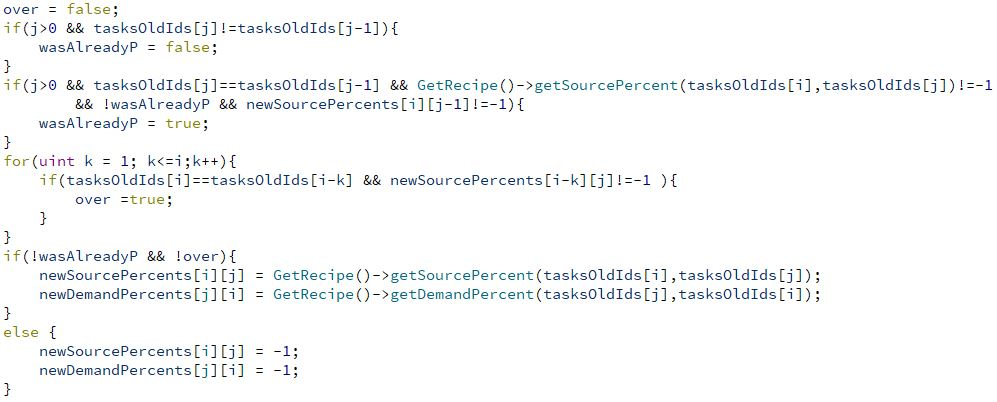
\includegraphics[scale=0.75]{MakeBatchFeltetelek}
\caption{Éleken lévő százalékok beállításának feltételei}
\label{MakeBatchFeltetelek}
\end{center}
\end{figure}
A könnyebb átláthatóság érdekében az ~\ref{MakeBatchPelda} ábrán látható egy példa. Két darab A terméket akarunk legyártani. Az adatok fájlból való beolvasása során az A1-es taszk megkapja a 0. azonosítót, az A2 pedig az 1. sorszámot. Mivel kettőt gyártunk le, ezért meghívódik a \textbf{MakeMultipleBatches} függvény, és újra kiosztja az azonosítókat, miközben létrehozta kellő számban az eredetiről lemásolt taszkokat. 
\begin{figure}[H]
\begin{center}
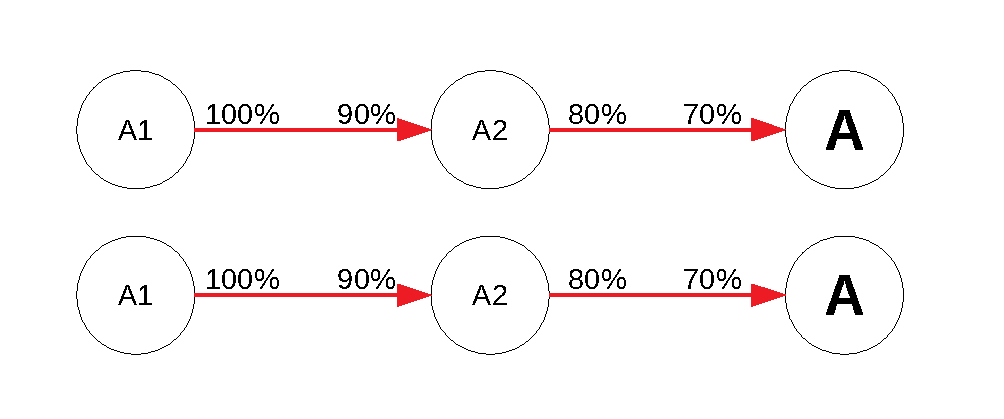
\includegraphics[scale=0.7]{MakeBatchPelda}
\caption{Példafeladat}
\label{MakeBatchPelda}
\end{center}
\end{figure}
Az új sorrend a következő táblázatban látható. Zárójelben látható, hogy az ~\ref{MakeBatchPelda} ábrán melyik sorban lévő recepthez tartozik.
\begin{table}[H]
  \begin{center}
  	\caption{A taszkokhoz tartozó azonosítók}
  	\captionsetup[table]{skip=10pt}
    \label{tab:table1}
    \begin{tabular}{|c|c|}
      \textbf{Taszk} & \textbf{Azonosító} \\     
      \hline
      A1 (első) & 0\\
      A1 (második) & 1\\
      A2 (első) & 2\\
      A2 (második) & 3\\
    \end{tabular}
  \end{center}
\end{table}
Azt nem lehet megengedni, hogy a 0 azonosítóval rendelkező taszk, a 3-as azonosítóval rendelkező taszk között él keletkezzen, mert nem az a kettő taszk tartozik egymáshoz. A példafeladatban látható, hogy egy él kezdő taszkjának, és annak a taszknak, amelybe érkezik, az azonosítójuk különbsége éppen annyi, amennyi terméket gyártani szeretnék. Jelen esetben kettő. 

\subsection{UpdateProfitBound függvény}
A függvény feladata, hogy kiszámolja az első S-gráfhoz tartozó korlátot, valamint minden egyes taszkhoz tartozó kapacitást is meghatározza. Legelső lépésben beállítja a taszkoknak az úgynevezett alap kapacitását. Ezt az alapján lehet meghatározni, hogy egyes berendezések, melyek a részfeladatot képesek elvégezni rendelkeznek kapacitással. Ezeket a bemeneti fájlból olvassa be a szoftver. Egy taszk kapacitását az összes, őt elvégezni képes taszk kapacitásának összege adja meg. Miután ez megtörtént következő lépés a kezdő csomópontok, taszkok megkeresése. Ez 2 \textit{for} ciklus segítségével történik, amelyekben vizsgáljuk, hogy az adott csomópont rendelkezik-e abba tartó, bementi éllel. Ha ilyen nincs akkor biztosak lehetünk benne, hogy az adott csomópont kezdő csomópont. Miután ezzel megvagyunk akkor megkeressük az előbb megtalált csomópontok szomszédjait. Ehhez egy \textbf{\textit{deque}} (double-ended queue), azaz kétvégű sort veszünk igénybe. Ennek előnye abban rejlik, hogy mind az elejére, mind a végéhez lehetséges elemet fűzni, illetve onnan eltávolítani. Ebbe a változóba tároljuk a kezdő csomópontok szomszédjait. Ismét két \textit{for} ciklus segítségével bejárjuk a taszkokat, amennyiben van köztük él, és még nem szerepel az adott taszk a \textbf{\textit{deque-ban}}, akkor beletesszük.

Mindezeket követően elérkezik az a rész, ahol a kapacitások meghatározása, felülvizsgálata következik. Egy \textit{while} ciklus segítségével minden \textbf{\textit{deque-ban}} szereplő elemet vizsgálunk, addig amíg az teljesen üressé nem válik. Először a \textbf{\textit{deque}} első elemét kivesszük belőle, majd egy \textit{for} ciklus segítségével ismét végighaladunk a taszkokon. Ha az éppen ciklusban lévő taszkból mutat él a \textbf{deque-ból} kivett taszkba, továbbá a taszknak, amiből az él indult, már korábban, a mostani függvény futása során, felül lett vizsgálva a kapacitása akkor lehet ellenőrizni a \textbf{\textit{deque-ból}} kivett taszk kapacitását. Ha az aktuálisan kiszámolt kapacitás nagyobb mint az eddigi, akkor a korábbi helyett az újat jelöljük ki a taszk kapacitásának. Ennek kiszámításhoz a következő képletet kell használni.
\begin{gather}
\scalebox{0.75}{$
\begin{align*}
\text{kapacitás}&= \text{előző taszk kapacitása}&*\frac{\text{előző taszkból felvett kapacitás mennyisége}}{\text{a mennyiég, amit az éppen vizsgált taszk feltud venni}}
\end{align*}$}	
\end{gather}
Abban az esetben, ha a kezdeti taszk még nem lett ellenőrizve, akkor nem lehet megvizsgálni az éppen kiválasztott taszkot, ezért visszatesszük a \textbf{\textit{deque}} végére. Ha viszont lehetséges volt és végbe is ment az adott taszk felülvizsgálata, akkor megkeressük ennek a csomópontnak a szomszédjait és hozzáfűzzük a \textbf{\textit{deque}} végéhez.

A függvény utolsó szakaszában történik meg a profit korlát meghatározása, kiszámolása. A korlátot azoknak a taszkoknak a kapacitása adja meg, amelyek a termékek előtti utolsó részfeladatok. Ezek megtalálása úgy történik, hogy \textit{for} ciklus segítségével bejárjuk a termékeket, valamit a taszkokat is. Ha valamelyik taszkból indul él egy termékbe, akkor a taszk kapacitását megszorozzuk a termékből származó jövedelemmel.

\subsection{UpdateProfitBoundFromTask függvény}
Ez a függvény feladatában hasonlít az előző pontban bemutatott \textbf{UpdateProfitBound} metódushoz. A taszkokhoz tartozó kapacitást, valamint a korlátot kell meghatároznia. Különbséget abban lehet felfedezni, hogy ennek a függvénynek nem kell a teljes S-gráfot bejárnia, az összes kapacitást nem szükséges újraszámolnia, hanem csak a paraméterben megadott taszkokhoz, és az ezt követő taszkokhoz tartozó kapacitásokat kell újraszámolnia. Az ezt követő taszkokat úgy kell értelmezni, hogy a megadott taszk szomszédjait, valamint azoknak a szomszédjait (így tovább egészen addig, amíg létezik egy szomszéd taszk) kell átvizsgálni és szükség esetén megváltoztatni, módosítani a kapacitásukat.

Az az előző pontban bemutatott függvénytől eltérően nem a S-gráf bemeneti csomópontjait reprezentáló taszkokat kell először megkeresni, hanem a paraméterlistában átadottat, valamint annak közvetlen szomszédjait. Ehhez is a \textbf{\textit{deque-t}} veszünk igénybe. Legelsőnek a az átadott taszk kerül bele, majd \textit{for} ciklus segítségével megkeresi annak szomszédjait, és ezeket is a \textbf{\textit{deque}} végéhez hozzáfűzi. Ezek után meg kell keresni a többi olyan taszkot is, amiknek a kapacitásukat újra át kell vizsgálni, és ha szükséges módosítani. Azt követően, hogy a két végű sor tartalmazza az összes átvizsgálandó taszkot megtörténik a tényleges kapacitás módosítás. Itt \textit{while} ciklus felhasználásával addig történik az ellenőrzés, amíg teljesen üressé válik a \textbf{\textit{deque}}. Ebből kivételre kerül a legelső elem, és megvizsgáljuk, hogy van-e ebbe tartó él, vagyis az S-gráf kezdő csomópontja vagy sem. Későbbiekben lesz szerepe ennek. Az éppen vizsgált taszk kapacitását átállítjuk nullára, majd a még hozzárendelhető berendezések kapacitásának összegét megkapja, mint az új érték. Amennyiben a taszknak nincs bejövő éle, akkor az imént meghatározott kapacitása megmarad, nincs szükség további ellenőrzésekre. Ez ellenben, ha van bemenő él, akkor még további feltételekre meg kell vizsgálni. Ha az a taszk, amelyből az él érkezik még nem ellenőrzött, akkor nem lehetséges a mostani taszk kapacitásának pontos meghatározása sem, ezért visszakerül a \textbf{\textit{deque}} végére. Azonban ha ellenőrzött a vizsgált taszkot megelőző részfeladat, akkor az előző pontban feltüntetett képlet szerint ki kell számolni a kapacitást. Ha ez nagyobb, mint a beállított akkor ezt kapja meg a taszk új értékként. Ellenkező esetben pedig marad a már meglévő érték. Ezeket követően szükséges még egy \textit{for} ciklus segítségével végigmenni a taszkokon, annak érdekében, hogy ha létezik megtalálja az összes szomszédját az imént vizsgált taszknak. Ha talált ennek megfelelő taszkot akkor a \textbf{\textit{deque}} végéhez hozzáadjuk.

Utolsó lépés a függvényben a profit korlát kiszámítása. Ez teljes mértékben megegyezik az előző pontban szereplő függvény befejező lépésével. Az S-gráfon a termék előtt szereplő utolsó részfeladat kapacitása szükséges a korlát kiszámításához. Azért, hogy megtaláljuk ezt a taszkot szükséges az, hogy két darab \textit{for} ciklus bejárja a termékeket és a taszkokat. Ha megtalálta akkor annak kapacitása és a terméken szerzett jövedelem szorzata megadja a korlátot.

\subsection{Egyéb új metódusok}
Az \textbf{IsProfitMaximization} függvény megadja, hogy az új módszer került meghívásra parancssori paraméterek által a megoldó szoftver indításakor. Olyan esetekben kerül meghívásra, amiket csak abban az esetben kell végrehajtani, ha az új, taszkok párhuzamos végrehajtására alkalmas módszert lett meghívva. Például a futás végén a fájlba írásnál kapacitásokat csak ennék a módszernél akarunk kiírni.

A másik egyszerűbb függvény a \textbf{GetTaskCapacity}. Paraméterként egy részfeladat azonosítóját várja, és ez alapján visszaadja az adott taszkhoz tartozó kapacitást.

\section{Argumentum hozzáadás}
Új módszer elkészítése miatt szükség volt új argumentumok hozzáadására a meglévők mellé. Az argumentumokat az \textbf{arguments.cpp} fájlban lehet elérni. Ez a fájl az \textbf{src\textbackslash solver} mappában található. Két argumentum került hozzáadásra. Az első \textbf{\textit{flexbatch}}, amely a \textbf{method} kapcsolóhoz tartozik. Ezzel a megoldómódszert lehet kiválasztani. A második új argumentum a \textbf{\textit{profit\textunderscore max}}, amely a \textbf{obj} kapcsolóhoz tartozik. Ez pedig a célfüggvényt reprezentálja.

\section{Megoldás fájlba írása}
Az új módszer kapcsolatos kapacitások kezelése eddig nem volt része a solver megoldó szoftvernek. Ez alól a fájlba történő kiírásuk sem kivétel, emiatt szükség volt a már meglévő kiírást elvégző függvény módosítására. A szóban lévő függvény a \textbf{WriteText}, amely \textbf{SGraph} típusú változót vár paraméterként. A függvény \textbf{solutionwriter.cpp} fájlban található míg a deklarációja a \textbf{solutionwriter.h} fájlban helyezkedik el. Ezeket a fájlokat a \textbf{src\textbackslash lib} mappában találhatjuk meg. 

Az eredetileg meglévő függvény a fájlba két elkülöníthető rész kiírását végezte. Az első volt, amely megmutatta az éleket. Ebbe beletartozik mind a recept, mind az ütemezési élek csoportja. Ezenfelül még megjelenik itt egy időérték, amely azt mutatja, hogy az adott taszkot, amelyből az él kiindul mennyi idő alatt lehet befejezni, elvégezni. Továbbá a boundot, korlátot is itt írja ki a fájlba a függvény. A második fele pedig az elvégzett feladathoz tartozó Gantt diagramot jeleníti meg karakteres formában. Ez megadja, hogy melyik taszkot, melyik berendezés végezi el, és, hogy ez mikor történik.

Az említett két rész közé került az általam elkészített kapacitások kiírására szolgáló rész. Pontosabban, mivel az új módszer kapacitás és jövedelem szorzataként adja meg a korlátot ezért, a rész a kapacitások utána jelenik ezentúl meg. Először a taszkok kapacitása kerül kiírásra. Ezeket követik a termékek, amelyekhez az utolsó taszk kapacitása és a termékből származó jövedelem adja meg az értéket. A korlát kiszámítása a termékekhez tartozó értékek összeadásával történik.
\chapter{Tesztelés}
Ebben a fejezetben az elkészített megoldó algoritmus tesztelését mutatom be, hogy az megfelelően, hiba nélkül képes a feladatokat megoldani.
A tesztelés a következő konfigurációval rendelkező számítógéppel történt:
\begin{itemize}
	\item Processzor: Intel i5-7200, 2,50 Ghz
	\item 8 GB RAM
	\item Operációs rendszer: Windows 10
	\item Fejlesztésnél használt szoftverek:
		\begin{itemize}
			\item Qt Creator 4.7.1
			\item Qt 5.11.2
			\item Boost Libraries 1.68.0
			\item Microsoft Visual C++ Compiler 15.0 
		\end{itemize}		 
\end{itemize}

Az S-gráf megoldó szoftvert parancssori paraméterek segítségével lehet működtetni. A különböző megoldó módszereket, amelyek megtalálhatóak a szoftverbe implementálva, más és más kapcsolók segítéségével lehet elérni, meghívni. Ezeknek listája megtalálható a \textbf{solver} mappában lévő \textbf{README.md} fájlban. Az általam megvalósított módszerhez a következő kapcsolókat mindenképpen használni kell, hogy a program hiba nélkül fusson és elvégezze az ütemezést:
\begin{itemize}
	\item \textbf{-i extended\textunderscore precedential.ods:} A bemeneti fájl elérési útvonalát kell megadni ezzel.
	\item \textbf{-o output.txt:} A kimeneti fájl elérési útvonala. Két fajta kiterjesztésű fájlt lehet megadni: \textbf{TXT} és \textbf{PNG}. Előbbi esetében a fájlba kerülnek az élek, mind a receptek, mind az ütemezési élek, valamint, hogy mennyi ideig tart a részfeladat befejezése, amelyből ezek kiindulnak. Ezenfelül a Gantt diagram karakteres formában is megjelenik. PNG kiterjesztésű fájl megadása esetén pedig kirajzolásra kerül egy Gantt diagram. Azonban, ha mindkét kiterjesztésű fájlra szükség van, akkor erre a \textbf{-g} kapcsoló segítségével van lehetőség. Ehhez a kapcsolóhoz kell a PNG kiterjesztésű fájl nevét megadni.
	\item \textbf{-m flexbatch:} Ezzel a kapcsolóval a megoldó módszert lehet kiválasztani. A \textit{felxbatch} határozza meg, hogy az általam megvalósított algoritmus kerüljön meghívásra.
	\item \textbf{--timehor:} Időhorizont megadása történik ezzel a kapcsolóval.
	\item \textbf{--obj profit\textunderscore max:} A célfüggvény kiválasztása, ebben az esetben az újonnan a megoldó szoftverhez hozzáadott profit maximalizálás kerül kiválasztásra.
	\item \textbf{--precycle off:} A precycle az ütemezés gyorsításra szolgál, mégpedig úgy, hogy előre lefut, és kört keres a gráfban. Az új módszer esetén hibásan működik, nem összeegyeztethető azzal, ezért szükséges a kikapcsolása.
	\item \textbf{--nopresolvers:} Hasonlóan az előzőhöz a presolver is az ütemezést gyorsítja, de nem egyeztethető össze az új megoldó módszerrel, emiatt kell mindenképpen inaktívvá tenni.
\end{itemize}

A ~\ref{tesztFeladat} ábrán látható mintafeladat alapján kerül bemutatásra a megoldó módszer. Két termékhez tartozó receptet látunk, amely a taszkokat, az ezeket megvalósítani képes berendezéseket, és az ehhez szükséges időt tartalmazza. Az éleken megfigyelhető még, hogy a kapacitások hány százaléka kerül továbbadásra, illetve a következő taszk által felvételre.
\begin{figure}[H]
\begin{center}
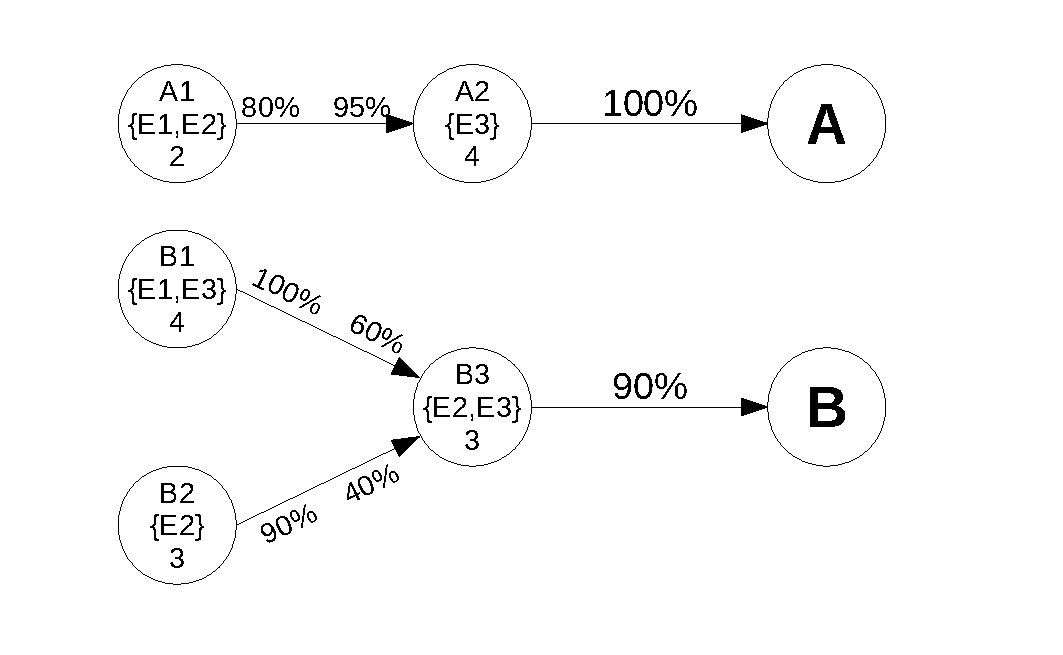
\includegraphics[scale=0.8]{tesztFeladat}
\caption{Tesztfeladat}
\label{tesztFeladat}
\end{center}
\end{figure}

\section{A tesztfeladat megoldása}
A módszer sajátossága, hogy a receptélekkel az egyes taszkok kapacitásának meghatározott százaléka hasznosítható. Ezeket a százalékokat a bemeneti fájlban kell megadni. A példafeladat a~\ref{bemenet1} ábrán megtekinthető bemeneti adatokkal rendelkezik. Az időhorizont a bemutatott mintafeladat során 15. Látható, hogy az egyes részfeladat által lehetséges kapacitásoknak nem a teljes mennyisége kerül tovább a következő taszkhoz. Az, hogy kisebb mennyiség kerül felhasználásra nagy mértékben befolyásolja a korlátot. Emellett az ütemezés megoldását is befolyásolja, mert emiatt lehetséges, hogy bizonyos berendezések nem végezhetik el az adott taszkot.

Az egyszerűség kedvéért a példában csak 2 darab termék receptje szerepel. Az A termék legyártásából származó jövedelem egy egység, a B termék esetén pedig 2 egység. A \textit{precendce} táblában látható, hogy a taszkok által elérhető mennyiségek nem 100 százalékban kerülnek további felhasználásra. Például az A1 és A2 taszkok esetében, az A1-es taszk mennyiségének 80 százaléka kerül továbbításra, illetve ennek a már kisebb mennyiségnek a 95 százalékát veszi fel az A2-es részfeladat. A \textit{proctime} táblán megtalálhatjuk, hogy melyik taszkot, melyik berendezés tudja elvégezni, valamint ezt mennyi idő alatt teszi.
 
\begin{figure}[H]
\begin{center}
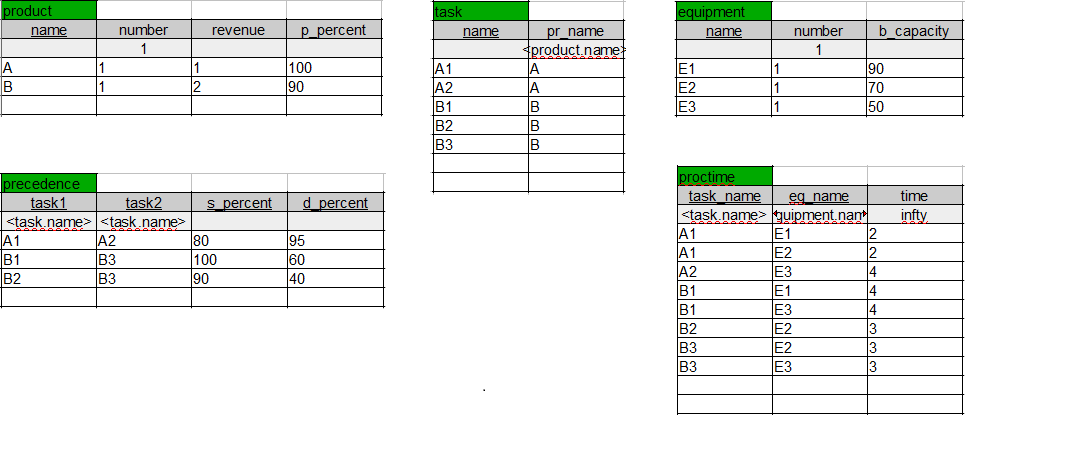
\includegraphics[scale=0.7]{bemenet1}
\caption{A tesztfeladat bemeneti adatai}
\label{bemenet1}
\end{center}
\end{figure}

A feladat megoldását tartalmazó TXT kiterjesztésű fájlt három darab elkülöníthető részre tudjuk felosztani. Az első része látható a~\ref{eredmeny1} ábrán. Az ábra elején az éleket találhatjuk meg, mégpedig olyan formában, hogy melyik taszkból melyik taszkba mutat. Továbbá láthatóak időértékek, amelyek megadják, hogy az élt megelőző részfeladatot mennyi idő alatt lehet elvégezni. Ez a rész tartalmazza mind a receptéleket, mind az ütemezési éleket. Úgy tudjuk ezeket elkülöníteni, hogy amelyikhez 0 időérték van rendelve, azok tartoznak az ütemezési élek csoportjához. Mivel az egyik termékből, nevezetesen az B-ből, több mint egy darabot gyártunk ezért megkülönböztetjük az egyes receptekhez tartozó feladatokat. Láthatunk B1-et és B1\textunderscore 2-t. Ugyanolyan típusú feladatról beszélünk, de különböző recepthez tartoznak, ezért kell megkülönböztetni egymástól ezeket.
 
\begin{figure}[H]
\begin{center}
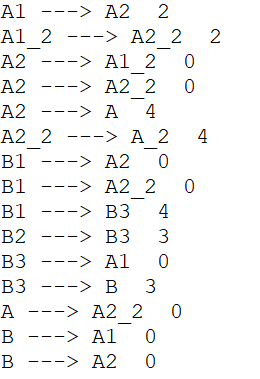
\includegraphics[scale=1]{eredmeny1}
\caption{A megoldást tartalmazó fájl első része}
\label{eredmeny1}
\end{center}
\end{figure}

A második részben a taszkok és a hozzájuk tartozó kapacitások, valamint a termékekhez tartozó kapacitások és a termékek előállításából származó jövedelem szorzata található. Ezeket követően szerepel a bound, a korlát, ami az adott feltételek és adatok mellett 482 lett. Ezt úgy kapjuk meg, hogy a termékekhez tartozó értékeket összeadjuk. Jelen példa esetében 3 érték kerül összeadásra, ezek a következők: A, B és B\textunderscore 2. Az A termékből származó jövedelem 50, a B és a B\textunderscore 2 termékek esetén 216. Ezeket összeadva kijön a 482. Ezek az értékek a~\ref{eredmeny2} ábrán megtekinthetőek.

\begin{figure}[H]
\begin{center}
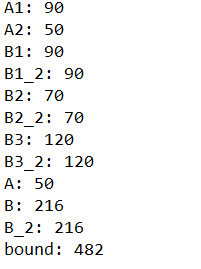
\includegraphics[scale=1.1]{eredmeny2}
\caption{A megoldást tartalmazó fájl második része}
\label{eredmeny2}
\end{center}
\end{figure}

Az utolsó szakaszban a Gantt diagram karakteres formában található meg. Látható, hogy vannak olyan taszkok, amelyeket több berendezés is el tud végezni. A \ref{eredmeny3} ábrán látható ez.

\begin{figure}[H]
\begin{center}
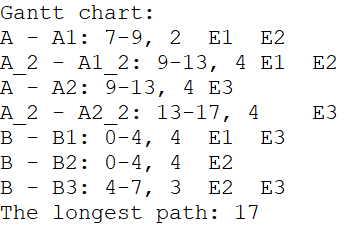
\includegraphics[scale=1]{eredmeny3}
\caption{A megoldást tartalmazó fájl harmadik része}
\label{eredmeny3}
\end{center}
\end{figure}

A \ref{kimenet} ábrán pedig a PNG kiterjesztésű fájl látható. Azonos színnel jelölt taszkok tartoznak egy termékhez. Ha az egyik termékből több példány készül, akkor a termékhez tartozó taszkok végéhez illesztett szám mutatja meg, hogy melyik termékhez tartoznak ezek. A diagramon könnyen észrevehető az új módszerben lévő újítás. A zölddel jelzett B3\_2-es taszk, valamint a kék színű B3-as taszk két berendezéshez, nevezetesen az E2 és az E3 berendezéshez is hozzá lett rendelve. 
\begin{figure}[H]
\begin{center}
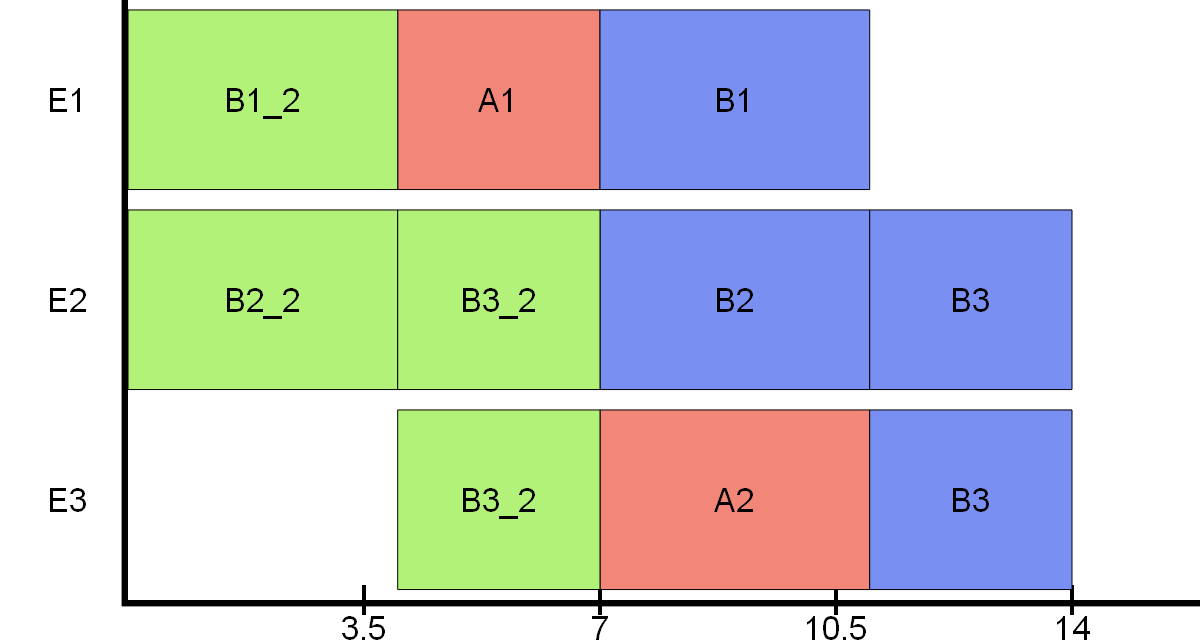
\includegraphics[scale=0.5]{kimenet}
\caption{A solver által elkészített Gantt diagram}
\label{kimenet}
\end{center}
\end{figure}

\section{A régi és az új megoldó összehasonlítása}
Ebben az alfejezetben az eddig meglévő throughput maximalizáló megoldót hasonlítom össze az általam létrehozottal. Ehhez \ref{tesztFeladat} ábrán látható feladatot veszem igénybe. Mivel ebben a feladatban a termékek változó batch mérettel rendelkeznek, ezért a régi megoldó módszerhez szükség van a 3. fejezetben bemutatott diszkretizálás végrehajtására. Ez látható a \ref{diszkretizalas} ábrán.

\begin{figure}[H]
\begin{center}
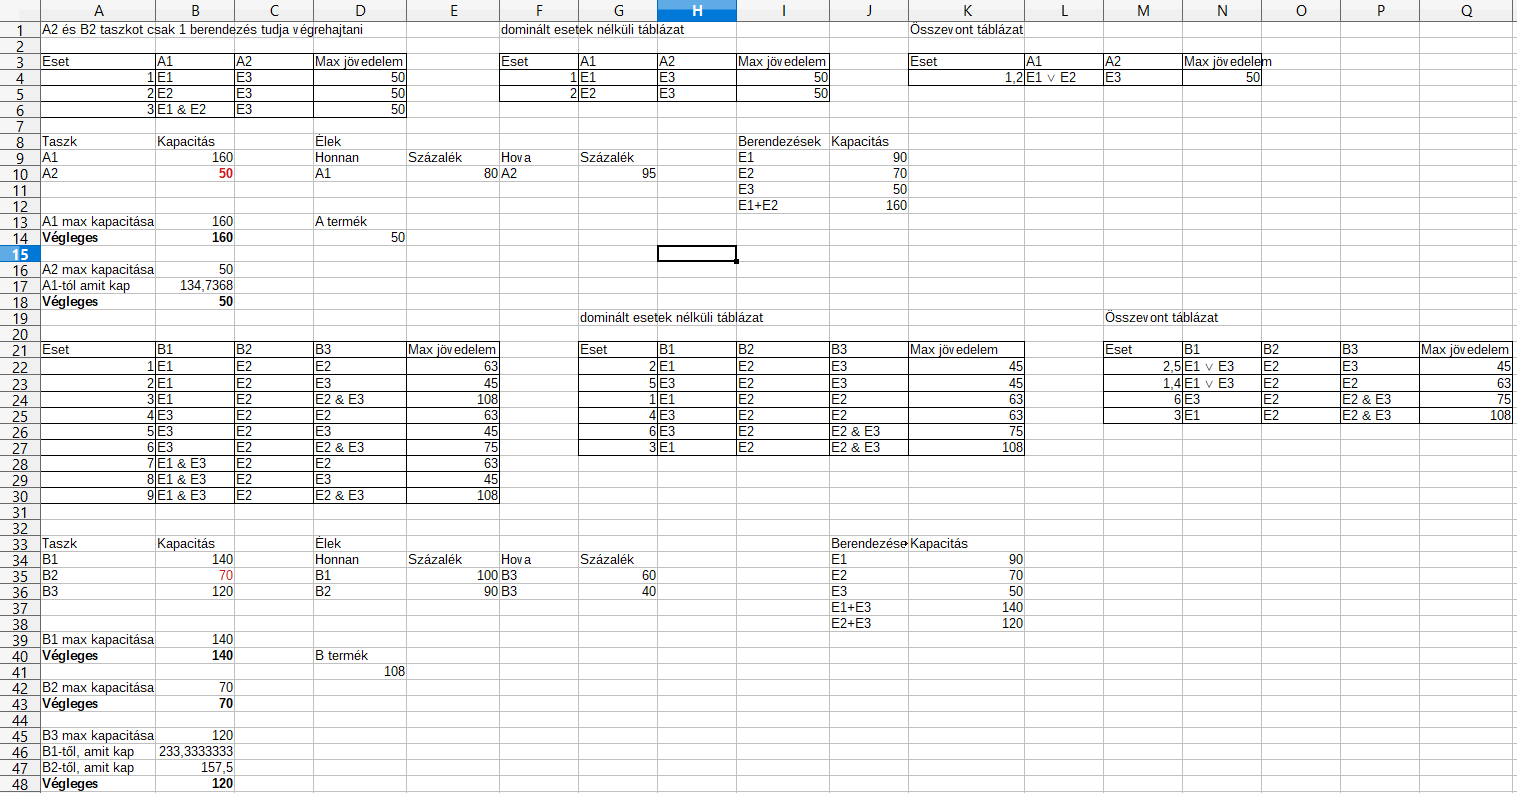
\includegraphics[scale=0.5]{diszkretizalas.png}
\caption{A \ref{tesztFeladat} ábrán látható feladat diszkretizálása}
\label{diszkretizalas}
\end{center}
\end{figure}

Ezt elvégezve eredményül azt kapjuk, hogy az A termék gyártása esetén mindenképpen 50 jövedelemre tudunk szert tenni. B termékhez viszont 4 különböző recept jött létre, amelyek mind eltérő jövedelmet biztosítanak. Ezek alapján felrajzolható a 4 gráf, amelyek a \ref{regi_grafok} ábrán láthatóak.
\begin{figure}[H]
\begin{center}
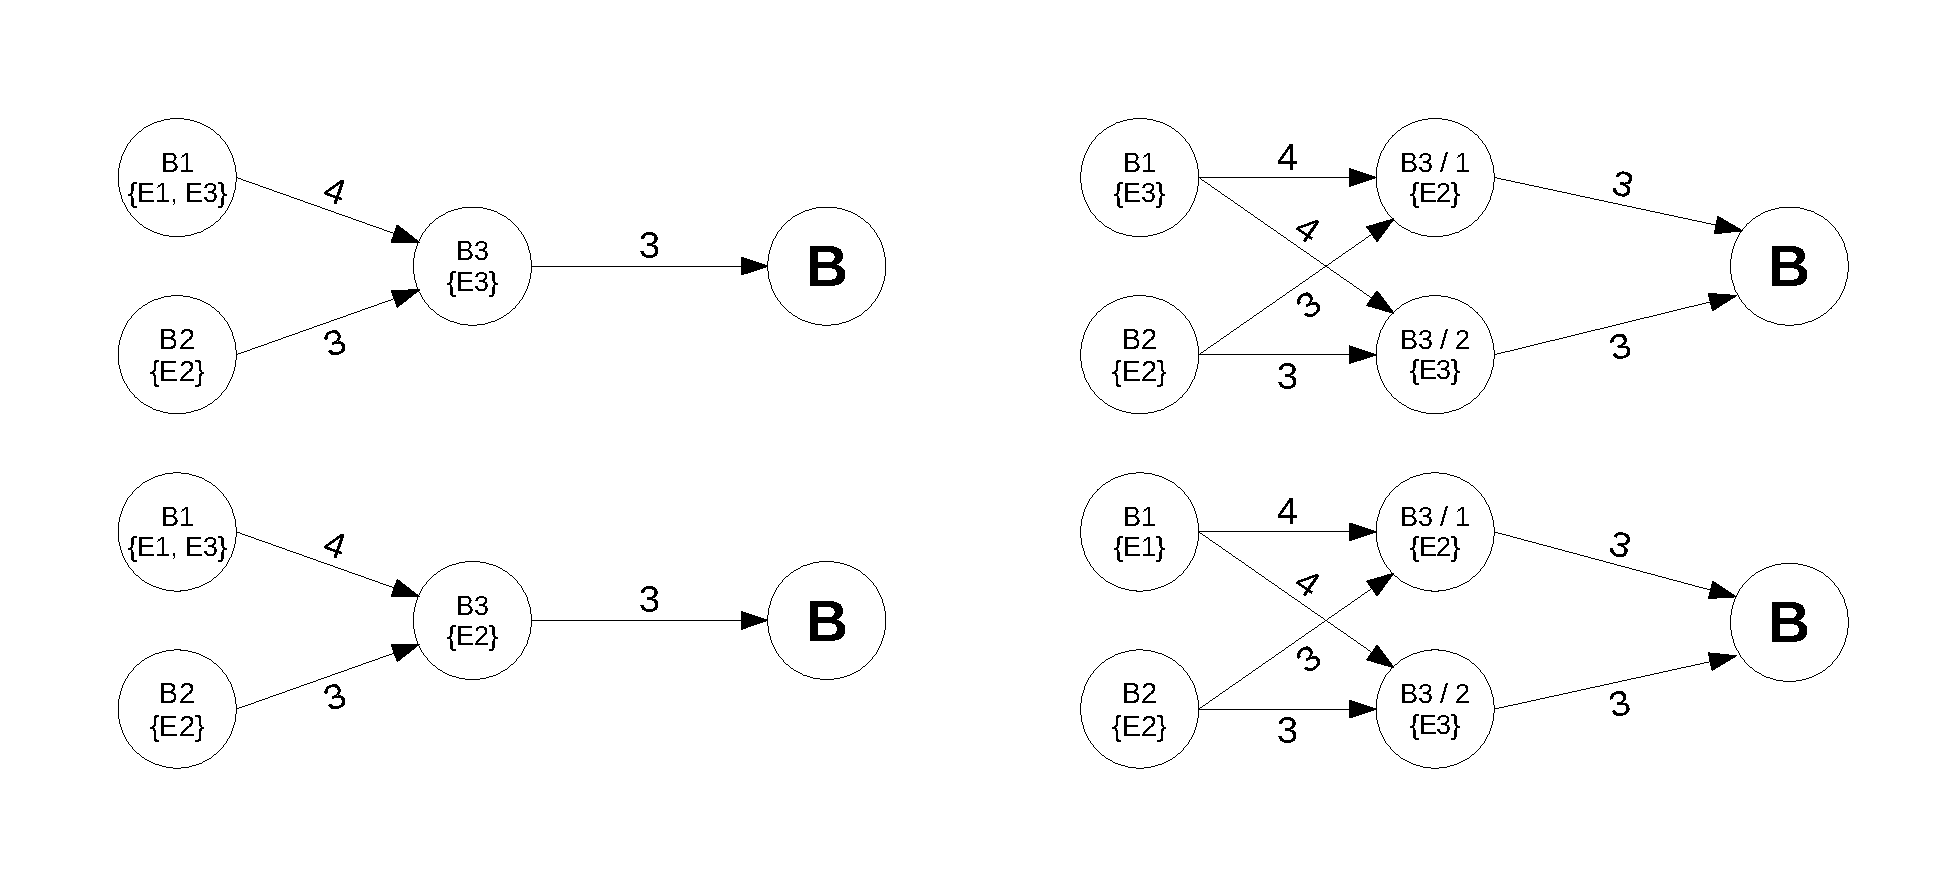
\includegraphics[scale=0.5]{regi_grafok}
\caption{Régi módszer esetén a B termékhez tartozó 4 gráf}
\label{regi_grafok}
\end{center}
\end{figure}
Az ábra bal oldalán szereplő gráfok megegyeznek a példafeladaton szereplő gráffal. Eltérés csak a taszkokat elvégezni tudó berendezésekben van. Azokat a  taszkokat, amelyeket 2 darab berendezés is el tud végezni, úgy kell figyelembe venni, hogy vagy az egyik vagy a másik berendezés végezi majd el az ütemezés után. A jobb oldalon látható, hogy a B3-as taszkból kettő darab lesz. Ezek az estek az jelentik, hogy mindkét berendezés elvégzi ezt a részfeladatot. A régi módszer esetén úgy tekintünk a termékekre, mintha 5 különböző termék lenne. Ezt az 1 darab A termék receptje és a 4 darab különböző B termék receptje adja meg. Ezek alapján elkészíthető a régi megoldóhoz szükséges bemeneti fájl, amely a következő ábrán látható. 

\begin{figure}[H]
\begin{center}
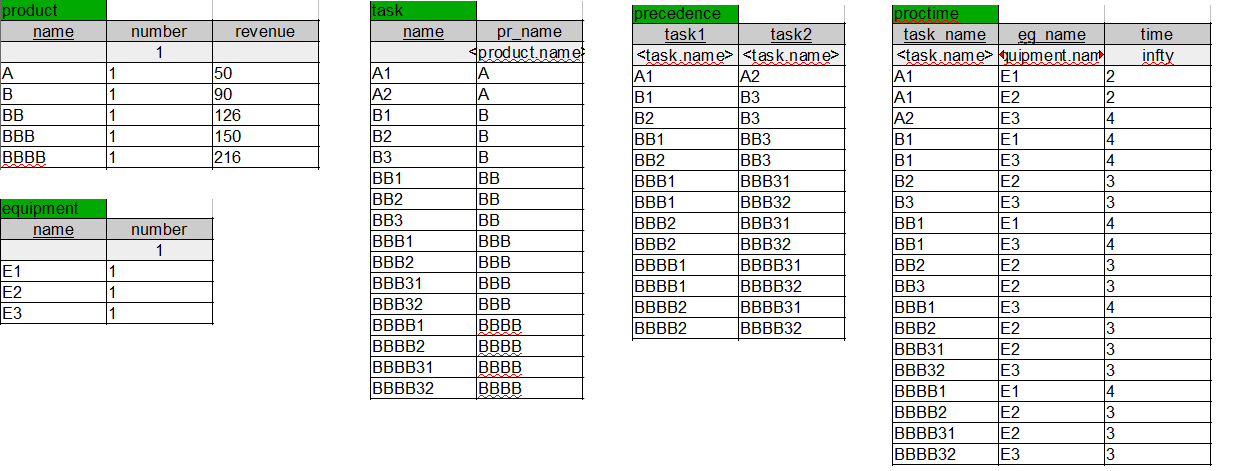
\includegraphics[scale=0.6]{regi_bemenet}
\caption{A régi megoldó bemeneti adatai}
\label{regi_bemenet}
\end{center}
\end{figure}

Látható, hogy ilyen típusú feladat esetében jóval több adat van a fájlban. Ennek az oka a több recept, ami több taszkot és élt jelent. Itt az 5 darab termék miatt egy 5 dimenziós teret lehet elképzelni. Az új megoldó módszernél ez csak 2 dimenziós tér lesz. Láthatjuk, hogy kevesebb dimenziót kell megvizsgálni, viszont egy dimenzión belül több számítást végez el az algoritmus a különböző hozzárendelési lehetőségek miatt. 

Az algoritmus lefutásának végeztével azt várjuk, hogy a régi és az új megoldó ugyanazt az eredményt szolgáltassa. Pontosítva a jövedelem mennyisége és a legyártott termékeknek meg kell egyezniük, a taszkok ütemezésétől azonban ezt nem várjuk el. A \ref{regi_kimenet} ábrán látható a régi megoldómódszer által elkészített Gantt diagram. Összehasonlítva a \ref{kimenet} ábrán látható diagrammal meg lehet állapítani azt, hogy mindkét esetben 2 B termék és 1 darab A terméket lehet legyártani a megadott időhorizonton belül. A másik fontos dolog, hogy a jövedelem is megegyezzen. Az új megoldónál ez 482 volt. A régi által nyújtott eredményben az A termék jövedelme 50, a két B termékből pedig olyanokat gyárt, amelyeknek 216 a jövedelme. Ezeket összeadva, 2 * 216 + 50, itt is kijön a 482. Az ütemezés során a taszkok sorrendje a két megoldó módszer esetén eltér, azonban ez nem hiba. Lehetnek olyan feladatok, ahol ez is teljes mértékben megegyezik.
\begin{figure}[H]
\begin{center}
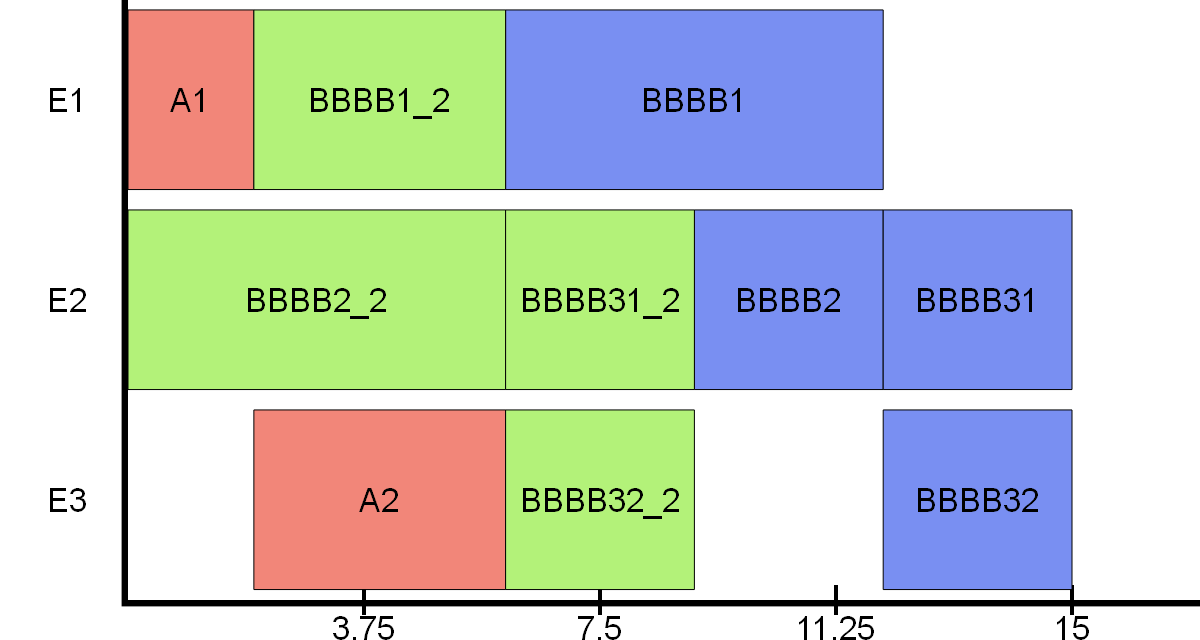
\includegraphics[scale=0.6]{regi_kimenet}
\caption{A régi megoldó által nyújtott Gantt diagram}
\label{regi_kimenet}
\end{center}
\end{figure}

\section{A megoldó módszerek sebessége}
A következő táblázatban a megoldó módszerek sebességének összehasonlítása látható. A régi módszerbe már több, különböző gyorsítási megoldás be van építve. Ezek közé tartozik a korábban már említett precycle és presolver. Az új módszer esetén ezek a gyorsítások jelen állapotban nem működnek. Egy másik kiemelt fontosságú gyorsítás a régi megoldó módszer esetében a revenue line. Ez alsó korlátként szolgál az egyes konfigurációkból származó jövedelmek összehasonlításához. Ennek segítségével, feladattól függően, nagy számú konfiguráció eltávolítható a keresési térből, így jelentősen csökkenthető a számítások mennyisége az ütemezés során. Az új módszer használata során azonban ezt nem vehetjük igénybe, mert nem egy egyenesen szerepelnek azok a konfigurációk, amelyek azonos jövedelemmel rendelkeznek. 

\begin{table}[H]
	\begin{center}
	\caption{Különböző módszerekkel megoldott feladatok összehasonlítása}
	\captionsetup[table]{skip=10pt}
	\label{teszteredmenyek}
\begin{tabular}{|l|l|c|c|c|c|}
\hline
                                                 & \multicolumn{1}{c|}{Megoldó módszer} & Futás ideje          & Time Horizon & Legyártott termék & Profit \\ \hline
\multicolumn{1}{|c|}{\multirow{9}{*}{\rotatebox{90}{Feladat 1}}} & Új                                   & 1,057 mp             & 15           & 1A+2B             & 482    \\ \cline{2-6} 
\multicolumn{1}{|c|}{}                           & Régi                                 & 0,149 mp             & 15           & 1A+2B             & 482    \\ \cline{2-6} 
\multicolumn{1}{|c|}{}                           & Régi (gy. n.)                        & 0,185 mp             & 15           & 1A+2B             & 482    \\ \cline{2-6} 
\multicolumn{1}{|c|}{}                           & Új                                   & 94,964 mp            & 20           & 1A+3B             & 698    \\ \cline{2-6} 
\multicolumn{1}{|c|}{}                           & Régi                                 & 8,17 mp              & 20           & 1A+3B             & 698    \\ \cline{2-6} 
\multicolumn{1}{|c|}{}                           & Régi (gy. n.)                        & 13,553 mp            & 20           & 1A+3B             & 698    \\ \cline{2-6} 
\multicolumn{1}{|c|}{}                           & Új                                   & \textgreater 8000 mp & 25           & 4B                & 864    \\ \cline{2-6} 
\multicolumn{1}{|c|}{}                           & Régi                                 & 705,439 mp           & 25           & 4B                & 864    \\ \cline{2-6} 
\multicolumn{1}{|c|}{}                           & Régi (gy. n.)                        & 1175,11 mp           & 25           & 4B                & 864    \\ \hline
\multirow{9}{*}{\rotatebox{90}{Feladat 2}}                      & Új                                   & 0,371 mp             & 15           & 2C+1D             & 188    \\ \cline{2-6} 
                                                 & Régi                                 & 0,07 mp              & 15           & 2C+1D             & 188    \\ \cline{2-6} 
                                                 & Régi (gy. n.)                        & 0,113 mp             & 15           & 2C+1D             & 188    \\ \cline{2-6} 
                                                 & Új                                   & 15,486 mp            & 20           & 3C+1D             & 252    \\ \cline{2-6} 
                                                 & Régi                                 & 1,306 mp             & 20           & 3C+1D             & 252    \\ \cline{2-6} 
                                                 & Régi (gy. n.)                        & 3,201 mp             & 20           & 3C+1D             & 252    \\ \cline{2-6} 
                                                 & Új                                   & 741,29 mp            & 25           & 3C+3D             & 360    \\ \cline{2-6} 
                                                 & Régi                                 & 58,28 mp             & 25           & 3C+3D             & 360    \\ \cline{2-6} 
                                                 & Régi (gy. n.)                        & 222,679 mp           & 25           & 3C+3D             & 360    \\ \hline
\multirow{6}{*}{\rotatebox{90}{Feladat 3}}                       & Új                                   & 14,78 mp             & 10           & 2H+2I             & 86     \\ \cline{2-6} 
                                                 & Régi                                 & 0,374 mp             & 10           & 2H+2I             & 86     \\ \cline{2-6} 
                                                 & Régi (gy. n.)                        & 0,381 mp             & 10           & 2H+2I             & 86     \\ \cline{2-6} 
                                                 & Új                                   & 44,693 mp            & 15           & 4I                & 94     \\ \cline{2-6} 
                                                 & Régi                                 & 0,985 mp             & 15           & 4I                & 94     \\ \cline{2-6} 
                                                 & Régi (gy. n.)                        & 0,806 mp             & 15           & 4I                & 94     \\ \hline
\end{tabular}
\end{center}
\end{table}

Ugyanaz a feladat 3 módszerrel került megoldásra. A régivel, amelyben szerepelnek a gyorsítások, ismét a régi megoldóval (régi gy. n.), de itt a precycle és a presolver gyorsítások nélkül, illetve az elkészített új megoldó módszerrel. Látható, hogy a régi módszerek gyorsabban találjak meg a feladat legjobb megoldását, mint az új a jelenlegi állapotában. Jövőbeni tervek közé tartozik a meglévő gyorsítások átalakítása, hogy kompatibilisek legyenek az új módszerrel is. Ezek megvalósítása után nagy csökkenés várható az új megoldó módszer futási idejében. 

A \ref{teszteredmenyek2} táblázatban olyan feladatok kerülnek összehasonlításra, amelyeknél egyfajta termék gyártható. Ugyanazon adatok alapján hasonlítottam össze a feladatokat, mint amelyek a \ref{teszteredmenyek} táblázatban láthatóak. Mivel ezeknél a feladatoknál csak 1 darab termék gyárható, ezért kevésbé összetettek. Az új megoldónak így mindössze 1 dimenziót kell bejárnia. Látható, hogy már vannak olyan feladatok, amelyeknél kisebb futási idő alatt megtalálta az optimális megoldást, mint a régi megoldó akár gyorsítással, akár anélkül. Ezen biztató jelek alapján várható, hogy gyorsítások implementálása után a nagyobb és összetettebb feladatok megoldásnál is jobb eredményeket érünk el az új megoldással.

\begin{table}[H]
\begin{center}
	\caption{Különböző módszerekkel megoldott feladatok összehasonlítása egy termékes feladatoknál}
	\captionsetup[table]{skip=10pt}
	\label{teszteredmenyek2}
\begin{tabular}{|l|l|c|c|c|c|}
\hline
                                                 & \multicolumn{1}{c|}{Megoldó módszer} & Futás ideje & Time Horizon & Legyártott termék & Profit \\ \hline
\multicolumn{1}{|c|}{\multirow{6}{*}{\rotatebox{90}{Feladat 4}}} & Új                                   & 0,029 mp    & 10           & 1A                & 30     \\ \cline{2-6} 
\multicolumn{1}{|c|}{}                           & Régi                                 & 0,055 mp    & 10           & 1A                & 30     \\ \cline{2-6} 
\multicolumn{1}{|c|}{}                           & Régi (gy. n.)                        & 0,057 mp    & 10           & 1A                & 30     \\ \cline{2-6} 
\multicolumn{1}{|c|}{}                           & Új                                   & 0,047 mp    & 12           & 2A                & 50     \\ \cline{2-6} 
\multicolumn{1}{|c|}{}                           & Régi                                 & 0,081 mp    & 12           & 2A                & 50     \\ \cline{2-6} 
\multicolumn{1}{|c|}{}                           & Régi (gy. n.)                        & 0,083 mp    & 12           & 2A                & 50     \\ \hline
\multirow{9}{*}{\rotatebox{90}{Feladat 5}}                       & Új                                   & 0,041 mp    & 10           & 2A                & 60     \\ \cline{2-6} 
                                                 & Régi                                 & 0,076 mp    & 10           & 2A                & 60     \\ \cline{2-6} 
                                                 & Régi (gy. n.)                        & 0,079 mp    & 10           & 2A                & 60     \\ \cline{2-6} 
                                                 & Új                                   & 0,152 mp    & 12           & 3A                & 90     \\ \cline{2-6} 
                                                 & Régi                                 & 0,236 mp    & 12           & 3A                & 90     \\ \cline{2-6} 
                                                 & Régi (gy. n.)                        & 0,265 mp    & 12           & 3A                & 90     \\ \cline{2-6} 
                                                 & Új                                   & 88,03 mp    & 15           & 5A                & 140    \\ \cline{2-6} 
                                                 & Régi                                 & 7,108 mp    & 15           & 5A                & 140    \\ \cline{2-6} 
                                                 & Régi (gy. n.)                        & 9,667 mp    & 15           & 5A                & 140    \\ \hline
\multirow{9}{*}{\rotatebox{90}{Feladat 6}}                       & Új                                   & 0,087 mp    & 10           & 2B                & 120    \\ \cline{2-6} 
                                                 & Régi                                 & 0,12 mp     & 10           & 2B                & 120    \\ \cline{2-6} 
                                                 & Régi (gy. n.)                        & 0,132 mp    & 10           & 2B                & 120    \\ \cline{2-6} 
                                                 & Új                                   & 1,71 mp     & 12           & 3B                & 180    \\ \cline{2-6} 
                                                 & Régi                                 & 0,872 mp    & 12           & 3B                & 180    \\ \cline{2-6} 
                                                 & Régi (gy. n.)                        & 1,01 mp     & 12           & 3B                & 180    \\ \cline{2-6} 
                                                 & Új                                   & 94,03 mp    & 15           & 4B                & 240    \\ \cline{2-6} 
                                                 & Régi                                 & 39,85 mp    & 15           & 4B                & 240    \\ \cline{2-6} 
                                                 & Régi (gy. n.)                        & 43,23 mp    & 15           & 4B                & 240    \\ \hline
\end{tabular}
\end{center}
\end{table}
\chapter{Összefoglalás}
A dolgozatomban a throughput maximalizálás szakaszos üzemű rendszerekben témakörrel foglalkoztam.
Először az ütemezéssel kapcsolatos irodalmat tanulmányoztam, amelynek során megismerkedtem az ipari környezetben használt ütemezési megoldó módszerekkel.
Ezek közül az S-gráf keretrendszer lett az, amely a dolgozatom alapját képezi.
Ezt követően megismerkedtem a makespan minimalizálás és a throughput maximalizálás algoritmusával.
Ezek megismerése adta meg az alapot, hogy elkészülhessen a flexibilis batch mérettel rendelkező feladatok megoldására alkalmas módszer.
Ez egy már meglévő S-gráf keretrendszert megvalósító szoftverbe történő implementálással valósult meg.
Az implementáció megvalósítását követően a bővített rendszert tesztelésnek vetettem alá.
A tesztelés eredményei azt mutatták, hogy a vizsgált feladatokra helyesen működik a program, mivel a régi megoldó módszerrel megegyező eredményeket szolgáltatott.
Ennek az új módszernek a segítségével idő spórolható meg az előfeldolgozó lépések során, mert már nem szükséges a diszkretizációs folyamat elvégzése.
Azonban a futási sebessége nem hozott minden feladat esetén jobb eredményeket, mint a régi megoldó módszer.
A jövőbeni tervek közé tartozik ennek az időnek a csökkentése.

Már felmerült több különböző gyorsítási ötlet.
Jelenleg a megoldó több batch esetén megvizsgál minden részproblémát, azokat is,
amelyekben a taszkok sorrendje megegyezik, csak egy másik, ugyanolyan termékhez tartoznak.
Ha már az első ilyen megvizsgált részprobléma során kiderül, hogy nem megvalósítható, akkor nagy mennyiségű számítást lehetne megspórolni, ha a többi részproblémát már a megoldó nem vizsgálná meg.
Ezen kívül érdemes lehet különböző stratégiákat megvizsgálni a berendezések kiválasztására.
Elképzelhető, hogy a jelenlegi kiválasztási stratégiánál található egy jobb.
Jelenleg a profitmaximalizáló algoritmus első futásakor a profit értéke 0.
Amennyiben a keresés a tengelyek mentén megtalált addigi legjobb profitról indulna, akkor elképzelhető, hogy bizonyos számú konfiguráció ütemezése feleslegessé válna, mert ebben az esetben az adott konfiguráció legjobb megoldása is kisebb profitot szolgáltatna, mint a tengelyeken megtalált legjobb megoldás.

\bibliographystyle{ieeetr}
\bibliography{Szakdolgozat}


\end{document}